%%%%%%%%%%%%%%%%%%%%%%
%%%%%% PACKAGES %%%%%%
%%%%%%%%%%%%%%%%%%%%%%

%%%%%%%%%%%%%%%%%
%%% Mandatory %%%
%%%%%%%%%%%%%%%%%
\documentclass[11pt,twoside,a4paper]{report}
\usepackage[DETI,newLogo]{uaThesis} %Later add ,final to remove 

%%%%%%%%%%%%%%%%
%%% Optional %%%
%%%%%%%%%%%%%%%%
\usepackage[english]{babel}
\usepackage{hyperref}
\usepackage{amsmath}
\usepackage{amssymb}
\usepackage{xspace}% used by \sigla
\usepackage{lipsum}
\usepackage[backend=biber, refsection=chapter, sorting=none, url=false]{biblatex}
\DeclareFieldFormat{pages}{#1}
\AtEveryBibitem{%
  \clearfield{note}%
}
\renewbibmacro{in:}{}
\AtEveryBibitem{\clearlist{language}}
\addbibresource{FinalReferences.bib}     %change to my bib.
\usepackage{csquotes}
\usepackage[acronym,nonumberlist, nopostdot]{glossaries}
\newglossary[tlg]{nomenclature}{tld}{tdn}{Nomenclature}
\usepackage{xcolor}
\usepackage{todonotes}
\usepackage[bottom]{footmisc}
\usepackage{amsmath}
\usepackage{xfrac}
\usepackage{mathdots}
\usepackage{yhmath}
\usepackage{cancel}
\usepackage{color}
\usepackage{siunitx}
\usepackage{array}
\usepackage{multirow}
\usepackage{amssymb}
\usepackage{gensymb}
\usepackage{tabularx}
\usepackage{booktabs}
\usepackage{caption,subcaption}
\usepackage{graphicx, epstopdf}
\usepackage{mathtools, nccmath}
\usepackage{pdflscape}
\usepackage{afterpage}
\usepackage{url}
\PassOptionsToPackage{hyphens}{url}
\usepackage[toc,page,title]{appendix}
\usepackage{listings}
\usepackage{placeins}
\lstset{
basicstyle=\small\ttfamily,
columns=fullflexible,
breaklines=true
}
\usepackage{pgfplots}
% and optionally (as of Pgf plots 1.3):
\pgfplotsset{compat=newest}
\pgfplotsset{plot coordinates/math parser=false}
\makeatletter
\g@addto@macro\bfseries{\boldmath}
\makeatother
%%%%%%%%%%%%%%%%%%%%%%
%%%%%%% MACROS %%%%%%%
%%%%%%%%%%%%%%%%%%%%%%

%%%%%%%%%%%%
% TOS
\setcounter{tocdepth}{2}
\setcounter{secnumdepth}{3}
% optional (comment to used default)
%   horizontal line to separate floats (figures and tables) from text
%\def\topfigrule{\kern 7.8pt \hrule width\textwidth\kern -8.2pt\relax}
%\def\dblfigrule{\kern 7.8pt \hrule width\textwidth\kern -8.2pt\relax}
%\def\botfigrule{\kern -7.8pt \hrule width\textwidth\kern 8.2pt\relax}

% custom macros (could also be defined using \newcommand)
\def\I{\mathtt{i}}         % one possible way to represent $\sqrt{-1}$
\def\Exp#1{e^{2\pi\I #1}}  % argument inside braces, i.e., "{}"
\def\EXP#1.{e^{2\pi\I #1}} % argument finishes when a full stop is encountered, i.e., "."
\def\sigla{\LaTeX\xspace}  % use as "blab blab \sigla blab blab (no need to do "blab blab \sigla\ blab blab"

\def\AddVMargin#1{\setbox0=\hbox{#1}%
                  \dimen0=\ht0\advance\dimen0 by 2pt\ht0=\dimen0%
                  \dimen0=\dp0\advance\dimen0 by 2pt\dp0=\dimen0%
                  \box0}   % add extra vertical space above and below the argument (#1)
\def\Header#1#2{\setbox1=\hbox{#1}\setbox2=\hbox{#2}%
           \ifdim\wd1>\wd2\dimen0=\wd1\else\dimen0=\wd2\fi%
           \AddVMargin{\parbox{\dimen0}{\centering #1\\#2}}} % put #1 on top #2

%%%%%%%%%%%%
% Mine
\def\ThesisYear{2020}
\def\myName{João André de Jesus Cruz}
\def\TituloTese{Telemetria para Vasilhame baseada em IoT}
\def\ThesisTitle{IoT-based Telemetry for Containers} %latter adapt

\setlength\bibitemsep{2.5\itemsep}        % increase space between bibliography entries

\emergencystretch=20em                     % Correct overfull h box

\setlength{\parskip}{0ex}

\newcommand{\figwidth}{0.6\textwidth}

\renewcommand{\arraystretch}{1.2}
\setlength{\tabcolsep}{12pt}

\DeclarePairedDelimiter{\nint}\lfloor\rceil
\DeclarePairedDelimiter{\nfloor}\lfloor\rfloor
\DeclarePairedDelimiter{\nceil}\lceil\rceil

\interfootnotelinepenalty=10000         % Change priority for footnotes

\newcommand{\todor}[1]{\todo[inline, color=red!40]{#1}}
\newcommand{\pathcos}[6]{\path (#1.east) to node [pathcos, color=#5, #6] {$\sfrac{#3\pi}{#4}$} (#2.west)}

\newcommand{\restor}[1]{\underset{*}{#1}}

\definecolor{lavenderblue}{rgb}{0.8, 0.8, 1.0}
\definecolor{aurometalsaurus}{rgb}{0.43, 0.5, 0.5}
\definecolor{bluegray}{rgb}{0.4, 0.6, 0.8}
\definecolor{glaucous}{rgb}{0.38, 0.51, 0.71}
\definecolor{coolblack}{rgb}{0.0, 0.18, 0.39}

\renewcommand\appendixname{Annexes}
\renewcommand\appendixpagename{Annexes}
\renewcommand\appendixtocname{Annexes}

%%%%%%%%%%%%%%%%%%%%
% load Glossary
\makenoidxglossaries
%\loadglsentries{glossary}

%%%%%%%%%%%%%%%%%%%%%%%%%%%%%%%%%%%
%%%%%%%%% BEGIN DOCUMENT %%%%%%%%%%
%%%%%%%%%%%%%%%%%%%%%%%%%%%%%%%%%%%
\begin{document}

%%%%%%%%%%%%%%%%%%%%%%%%%%%%%%%%%%%%%%%%%%%%%%%%%%%%%%%%%%%%%%%%
% cover, back cover, Jury, acknowledgment, key words, summary
% CoverPage
\TitlePage

  \HEADER{\BAR}
         {\ThesisYear}
  \TITLE{\myName}
        {\TituloTese}
        {\ThesisTitle}
\EndTitlePage
\titlepage\ \endtitlepage % empty page


%
% Initial thesis pages
%

\TitlePage
  \HEADER{}{\ThesisYear}
  \TITLE{\myName}
        {\TituloTese}
        {\ThesisTitle}
  \vskip 15mm
  \TEXT{}
       {Dissertação apresentada à Universidade de Aveiro para cumprimento dos requesitos necessários à obtenção de grau de Mestre em Engenharia Eletrónica e Telecomunicações, realizada sob a orientação científica do Professor Doutor Pedro Nicolau Faria da Fonseca, Professor Auxiliar e coorientação do Professor Doutor Paulo Bacelar Reis Pedreiras, Professor Auxiliar do Departamento de Eletrónica, Telecomunicações e Informática da Universidade de Aveiro}
\EndTitlePage
\titlepage\ \endtitlepage % empty page

\TitlePage
     \vspace*{55mm}
     \TEXT{\textbf{o júri~/~the jury\newline}}
          {}
     \TEXT{presidente~/~president}
          {\textbf{Prof. 
          }\newline {\small
          Professor }}
     \vspace*{5mm}
     \TEXT{vogais~/~examiners committee}
          {\textbf{Prof. Doutor Frederico Miguel do Céu Marques dos Santos}\newline {\small
          Professor Adjunto do Instituto Superior de Engenharia de Coimbra}}
     \vspace*{5mm}
     \TEXT{}
          {\textbf{Prof. Doutor Pedro Nicolau Faria da Fonseca}\newline {\small
          Professor Auxiliar da Universidade de Aveiro (Orientador)}}
\EndTitlePage
\titlepage\ \endtitlepage % empty page

\TitlePage
  \vspace*{55mm}
  \TEXT{\textbf{agradecimentos~/\newline acknowledgements}}
       {Em primeiro lugar e especialmente, aos meus pais por todo o apoio e pela oportunidade de estudar nesta instituição. Às minhas irmãs e à minha restante família pelo apoio que sempre me deram. \newline A todos os amigos e colegas que estiveram presentes ao longo deste percurso. \newline Ao Diogo, Edgar, Kevin e Miguel. \newline  Por fim, aos professores Pedro Fonseca e Paulo Pedreiras pela oportunidade de trabalhar nesta dissertação, pela orientação e apoio no desenvolvimento da mesma.}
\EndTitlePage
\titlepage\ \endtitlepage % empty page

\TitlePage
  \vspace*{55mm}
  \TEXT{\textbf{Palavras-Chave}}
       {Gases de petróleo liquefeito, FFT, Acelerómetro, Piezoeléctrico}
  \TEXT{\textbf{Resumo}}
       {Esta dissertação apresenta um estudo efectuado com o intuito de desenvolver um dispositivo capaz de medir a quantidade de gás líquido dentro de uma garrafa, de forma não evasiva. A investigação realizada resultou na identificação de diferentes métodos de medição de nível, como por exemplo a medição do peso, a análise das vibrações resultantes da estimulação externa, entre outros. Da investigação para a escolha do método de identificação de nível de líquido, optou-se por desenvolver o trabalho com base na análise das vibrações produzidas quando estimulada a garrafa.}
  \TEXT{}
       {O trabalho dividiu-se em diferentes objetivos, todos com vista ao desenvolvimento de um dispositivo que se enquadre no propósito. Inicialmente identificou-se a resposta da garrafa a um estimulo externo, ao analisar a sua resposta em frequência, para tal recorreu-se a um microfone para captar a mesma. De seguida procedeu-se à implementação e validação da FFT em um microcontrolador de pouco consumo energético, com o intuito de verificar a viabilidade de fazer a análise em frequência no microcontrolador. Após isto o trabalho centrou-se na seleção e testes a sensores, para substituir o microfone utilizado inicialmente, para isso foi utilizado um acelerómetro e um piezoeléctrico. Por fim procedeu-se ao desenvolvimento de um algoritmo de identificação de nível, com base nas vibrações captadas pelos sensores, que permita distinguir as diferentes garrafas utilizadas em testes.} 
\EndTitlePage
\titlepage\ \endtitlepage % empty page
%%English version
\TitlePage
  \vspace*{55mm}
  \TEXT{\textbf{Keywords}}
       {Liquefied petroleum gas, FFT, Accelerometer, Piezoelectric}
  \TEXT{\textbf{Abstract}}
       {This dissertation presentes the study made with the intent of developing a device capable of measuring the amount of liquid gas inside a bottle, in a non evasive way. The realized investigation resulted in the identification of diferent methods to measure the level, as for example the weight measure, the vibrations analisys from the external stimulation, among others. From the investigation to select the liquid level identification, it was chosen to develop the work based on the analisys of the vibrations produced when stimulated.}
  \TEXT{}
       {The work was divided with different objectives, all of them with the development of a device that fits in the purpose in perspective. Initially was identify the response of the bottle to a external stimulation, by the analisys of the frequency response, for that a microphone was used to capture the response. This was proceeded by the implementation and validation of the FFT in a low poer microcontroller, with the intent to verify the viability of the frequency analisys in the microcontroller. After this, the work focused in the selection and the test of sensors, to substitute the microphone inicially used, for that a accelerometer and a piezoeletric was chosen. Finally, was developed an algorithm to the level identification, based on the vibrations captured with the sensors, that allow to distinguish between the three bottles used in the tests.}
\EndTitlePage
\titlepage\ \endtitlepage % empty page



%%%%%%%%%%%%%%%%%%%%%%%%%%%%%%%%%%%%%
% Tables of contents, of figures, ...
\pagenumbering{roman}
\tableofcontents

\cleardoublepage
\listoffigures
\addcontentsline{toc}{chapter}{\listfigurename}

\cleardoublepage
\listoftables
\addcontentsline{toc}{chapter}{\listtablename}

\cleardoublepage
% \printnoidxglossary[type=\acronymtype]
\addcontentsline{toc}{chapter}{\acronymname}

\cleardoublepage
% \printnoidxglossary
% \addcontentsline{toc}{chapter}{\glossaryname}

\cleardoublepage
% \printnoidxglossary[type=nomenclature,title=Nomenclature]
\addcontentsline{toc}{chapter}{Nomenclature}

%%%%%%%%%%%%%%%%%%%%%%%%%%%%%%%%%%%%%
% Introduction
\todo[inline,color=green!40]{*Add References chapter at the end}
\todo[inline,color=green!40]{*1-Introduction Chapter Incomplete}
\cleardoublepage
\pagenumbering{arabic}
\chapter{Introduction}
\todo[inline,color=red!40]{*Change scope}
%%%%%%%%%%%%%%%%%%%%%%%%%%%%%%%%%%%%%%%%%%%%%%%%%%%%%%%%%%%%%%%%%%%%%%%%%%%%%%
\section{Background and Motivation} %% Change it latter
%% commands \gls, \Gls, \glspl and \Glspl used in glossary
%% command \footnote used in foot notes 

Energy plays an important role in our modern lifestyle and the development process of any country. And studies shown a strong correlation between the energy production/consumption and the economic/scientific development. Back in a couple of centuries ago, the primary source of energy was wood, as the industrialization evolved the needed of energy sources with higher energy efficiency rates\cite{demirbasGlobalEnergySources2004}. The first successor was charcoal followed, a few years latter by oil and \acrshort{lpg}(\acrlong{lpg}). Compared with the other energy sources, \acrshort{lpg} burns very efficiently, realizing smaller amounts of pollutants gases. For example to produce the same amount of energy produced by 1Kg of \acrshort{lpg}, burning it in a cookstove, it would be need approximately at least 2.5Kg of charcoal and 21.Kg of raw wood~\cite{File201403Multiple}. 

\acrshort{lpg} if the second biggest, non-renewable, source of energy in the world, with different consumption areas, as domestic, auto, industrial and agriculture. With the biggest consume in a domestic level, since is used to heating and cooking, with various types of \acrshort{lpg} produced by the extraction of natural gas, oil extraction and oil refining, the most common used in house appliances are propane, butane and natural gas\cite{LiquefiedPetroleumGas}. More recently the energy sources have been replaced with renewable energy, to decrease the environmental impact and however \acrshort{lpg} has bigger impact, doesn't seem that it won't be replaced by other sources of energy, since recent studies developed what can be considered a renewable method of biosynthesis propane gas~\cite{kallioEngineeredPathwayBiosynthesis2014b}, commonly used in house appliances.   

The \acrshort{lpg} use in house appliances, usually is made via pluming systems in the cities, were the agglomeration of population is bigger, which turns the installation of gas pipelines more economic viable when compared with other regions. For smaller villages the solution for the \acrshort{lpg} distribution is based on the gas cylinders, which is divided in two main distribution system, \acrlong{cccm}, where the final consumer is responsible for refueling the cylinder, most commonly used in cars, and \acrlong{bcrm}, where the final consumer only exchange a empty cylinder for a full one, being the supplier responsible for its refill, which require additional logistics for the suppliers distributions systems. For the second, it would be interesting for the suppliers and the cylinder retailers, to know the amount of gas in the cylinder of each final consumer of a certain region of supply.

This motivated a research in a accurate method of measuring the amount of gas in a \acrshort{lpg} cylinder and transmit that information to the supplier, taking advantage of the technology and using a \acrshort{iot}, as a way to transfer the information, suppliers would be able to efficiently plan their distribution routes. 

In a initial stage different methods of measuring the level of gas in a \acrshort{lpg} cylinder will be explored, and the the work developed is based in one of those methods, all the details will be explained further in the document.

\section{Scope}
%\todo[inline,color=red!40]{Rewrite this, I don't like}
This work explores the possibility of develop a device capable of measuring the liquid gas inside a bottle in a non evasive way. 

Initially will be made a study of devices with similar purpose, this will allow the proposal of an architecture to a system capable of measure, process and identify the liquid gas inside the cylinder. This must be followed by the implementation of the proposed solution. In the end will be performed individual tests to each piece of the system, concluding with the test for the identification. 
%%Older
%In order to develop a system that is robust/precise and featuring a system capable of communicate with the supplier and transmit the necessary information. A previous research must be made, to find similar work developed in the same field.

%Taking in consideration previous works, the identification of the measuring method must be made, looking to the pros and cons of all methods, and selecting the one that can provide the robustness and precise needed. For the communication system, should be based in IoT, and its range should cover most of the territory, to allow the information transfer of each LPG cylinder.

%The final device, should include all of the features mentioned, and take into consideration the components/development cost, making it relatively cheap to produce and within the business plan of the producer, and affordable for the final user.

\section{Outline}
This dissertation is divided in seven different chapters. The first chapter gives a general overview of the motivation behind the dissertation and defines the objectives to archive in the development of the work. 

The second starts by some background information, about previous works with similar purpose and a brief explanation of of the theoretical components behind the work to develop. This chapter is the basis to define a solution to approach the problem presented.

The third is where is defined the approach to solve the presented work, it is presented all the necessary elements of the system to developed and a general system architecture suggested.

The fourth and fifth chapters is were is defined the each one of the elements, the first relative to the physical, or hardware, elements that will be part of the system and the second is defined concerns about the software and the details of the integration of the hardware with the software.
The sixth chapter, is dedicated to present the different tests, their results and their analysis. The tests performed will serve as a basis to the continuation and integration of all parts in to what was proposed in chapter three. 

The work is finishes with Chapter seven, where are made some final considerations about the developed work, as well as suggestions for the future work.
\clearpage
%\printbibliography[heading=subbibliography]
%\addcontentsline{toc}{section}{References}

%%%%%%%%%%%%%%%%%%%%%%%%%%%%%%%%%%%%%
% AV1 Video Codec
\cleardoublepage
%To do notes colors meaning
%red - Not started
%yellow - In progress
%light blue - Done, under approval
%Green - Done and approved
\chapter{State of the Art}\label{chap:stArt}
%%Section To do
\todo[inline,color=blue!40]{*1-The LPG cylinder}
\todo[inline,color=blue!40]{*2-Measuring/Stimulation Tecniques}
\todo[inline,color=blue!40]{*3-Signals and systems - missing images}
\todo[inline,color=blue!40]{*4-LPG cylinder Model}
\todo[inline,color=blue!40]{*5-Vibration Sensors}


%----------------------------------------Section 1-----------------------------------
%Introduction to the chapter
In this chapter will be presented several topics, related with the LPG cylinder, previous works, systems concepts important for the work and sensors for it. To better understand the system to which is being design a device to measure the liquid level, in necessary to understand the constitution of the LPG cylinder and what are the variables that vary in the system. After it, is important to make a background search in previous works and their approaches, to understand if it's feasible and what is the approach to be taken. When selecting the technique to use for the purpose of the solution and before getting into the theoretical details of it, is necessary to understand everything that is related to the system, in a engineering point of view. In the end, will be presented different sensors, that can be used according to the type of measurements pretended in future product.     
\section{The LPG cylinder}
%Subsections to do
The LPG cylinders commonly used in house appliances, usually came in different weight types, that are change according to the cylinder construction, the supplier, his application and composition of gas that is being healed inside the container. One thing that is similar is the state of the gas under certain circumstances, for instance the boiling point of LPG is around -42ºC, which means that under ambient pressure/temperature the gas is in his gaseous state. 

Usually inside a LPG cylinder, the gas is kept in a liquid and gas form, in a percentage of around 80\% and 20\%, respectively, with a constant pressure, this percentage allows, when the external temperature rises, affecting the internal temperature, for both gas and liquid to expand until a certain limit, without compromise the safety of the use of the cylinders.
\begin{figure}[!htb]
    \centering
    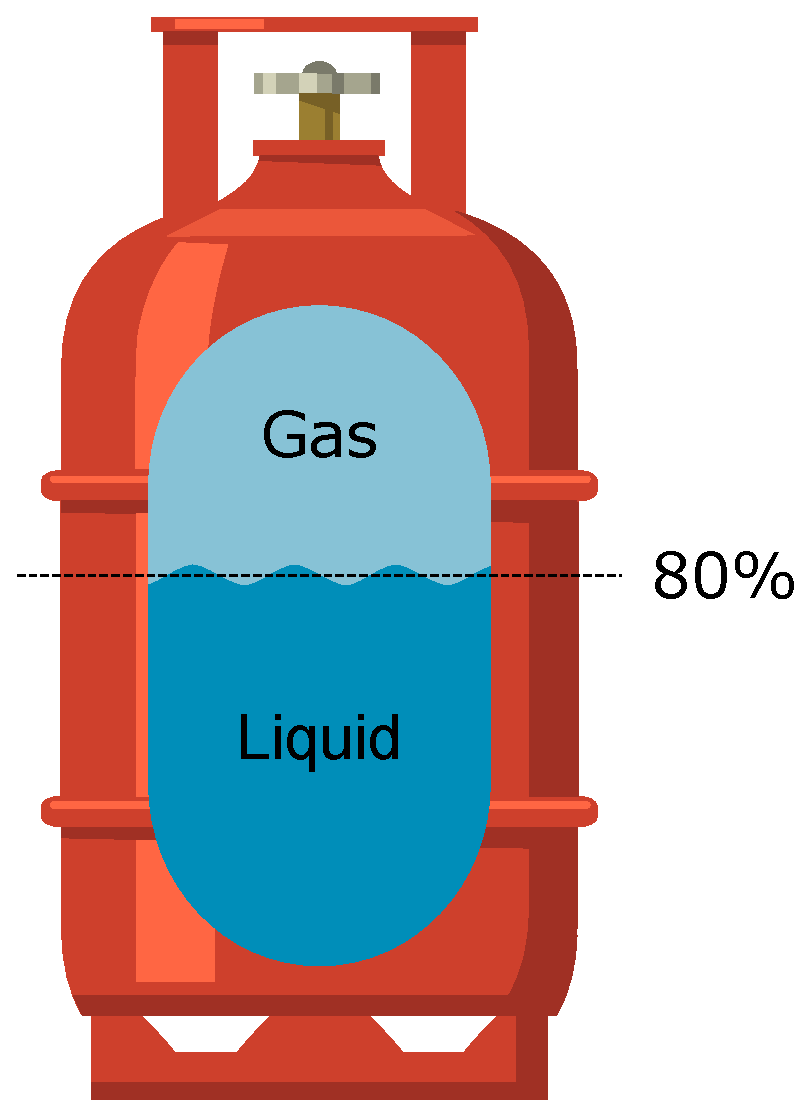
\includegraphics[width=0.25\textwidth]{Chapters/2CHP/Diagrams/bottleBaseliqGas.eps}
    \caption{LPG cylinder internal state composition}{}
    \label{fig:intcomplpg}
\end{figure}

When the cylinders are empty and need to be filled, there is a direct relation between the amount of pressure, needed to fill the cylinders, and the temperature of the gas, the higher the temperature of the gas the higher is the pressure needed to fill the cylinder, this process of turning the LPG in a gas form into a liquid by pressurizing it, is called liquefaction. Another relation that must be taken into consideration, is the weight of the cylinder and the amount of liquid LPG, when the cylinder valve is open and LPG gas is released, the liquid LPG is turns into gas in order to keep a balance of pressure inside the cylinder, since that for the same pressure the density of the LPG liquid is higher then the density of the LPG gas, when the amount of liquid LPG decreases the weight of the cylinder also decreases \cite{WhatAreProperties} \cite{PropaneDensitySpecific}.

%%Correct about gas pressure inside the bottle

%----------------------------------------Section 2-----------------------------------
\section{Measuring/Stimulation Techniques}\label{sec:measStim}
\subsection{Measuring Techniques}
As the LPG cylinder content is divided in two physical states, liquid and gaseous, over the years several techniques have been used and improved in measuring the liquid level, which is how is determined the amount of LPG in the cylinder, some of the different techniques used are based on the same method. Those methods are usually split in two different categories, contact and contactless. Contact measuring methods usually include, mechanical, electrical or pressure sensing devices. In this methods the sensors are in direct contact with the liquid. In contactless, the methods used usually are more complex to process, when compared with contact methods. In this case the methods of measuring are mainly through optical, ultra-sound, vibration and weight analysis\cite{nakagawaContactlessLiquidLevelMeasurement2013a}. 
\begin{figure}[!htp]
    \centering
    \begin{subfigure}{0.15\textwidth}
        \centering
        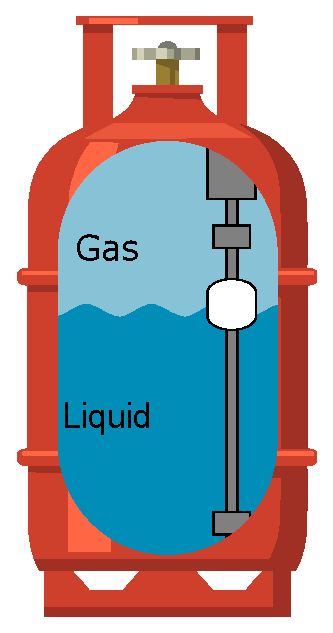
\includegraphics[width=\linewidth]{Chapters/2CHP/Diagrams/bottleBasefluctuator.eps}
        \caption{}{}
        %\label{subfig:g1lines}
    \end{subfigure}
    \begin{subfigure}{0.15\textwidth}
        \centering
        \includegraphics[width=\linewidth]{Chapters/2CHP/Diagrams/bottleBaseelectrode.eps}
        \caption{}{}
        %\label{subfig:g2lines}
    \end{subfigure}
    \begin{subfigure}{0.15\textwidth}
        \centering
        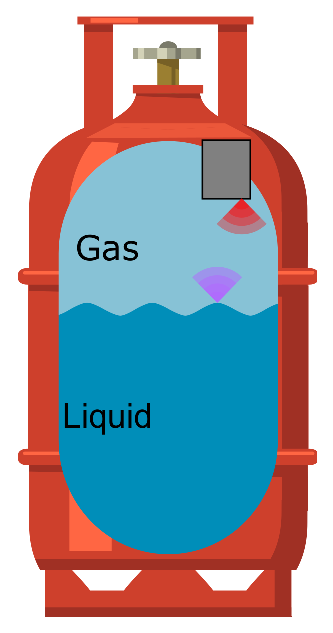
\includegraphics[width=\linewidth]{Chapters/2CHP/Diagrams/bottleBaseultrasound.eps}
        \caption{}{}
        %\label{subfig:g3lines}
    \end{subfigure}
    \begin{subfigure}{0.15\textwidth}
        \centering
        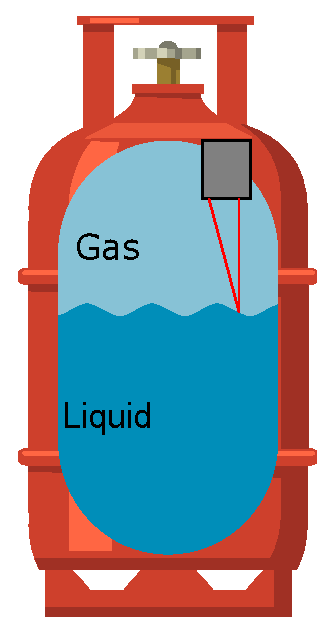
\includegraphics[width=\linewidth]{Chapters/2CHP/Diagrams/bottleBaseoptical.eps}
        \caption{}{}
        %\label{subfig:g4lines}
    \end{subfigure}
    \caption{Different LPG cylinder to used to compare the relation between Frequency and Weight for different models}{\citeauthor{wuLiquidLevelDetector2014b}}
     %\label{fig:noise}
 \end{figure}
Taking in consideration the fact that a LPG cylinder is opaque and isolated, some of the methods can't be used in the process, for instance, a mechanical float-type isn't a suitable solution to use inside the cylinder, or in the same way to use an electrode, as a electrical method, in these cases the device would require to be installed inside the cylinder during his fabrication process, possibly implying the substitution of the current cylinders. In the same way, in contactless methods, the use of different optical techniques and the use of of ultra-sound, would face the same problem mentioned with the contact methods, being also discard as a suitable method in this situation. 

From previous research, some work has already been developed with the purpose of measuring the amount of liquid gas inside a LPG cylinder. Being the techniques used based on the methods presented above.
%Based on the pressure
In a work from \citeauthor{baigAccurateMeasurementPressure2008b} a pressure sensing device was developed, with the final appliance to a LPG cars, but with the possibility of apply in other circumstances. The device uses the pressure variation to move a magnet and using a Hall Effect sensor, with a fixed position, this motion produces a linear change of the voltage in the sensor, giving an accurate method of measuring the amount of gas in the LPG cylinder, in this case\cite{baigAccurateMeasurementPressure2008b}. 
%Based on the weight
A common method of evaluate the amount of gas inside a LPG cylinder, is based on the weight change of the cylinder, that decreases with the consumption of liquid gas. As an example, the work developed by \citeauthor{dasilvamedeirosSmartgasSmartPlatform2017a}, \citeauthor{shresthaIoTBasedSmart2019a} or \citeauthor{shinganSmartGasCylinder2017a} have similar approaches to measure the amount of liquid gas inside the LPG cylinder. There is various works based on this technique since is very simple to implement and very precise, it only requires a load cell, a amplifier, a microcontroller and a method to display the results, and unless there is a huge change in the external temperature, the density of the gas won't be much affected and thus not affecting the weight of the bottle \cite{dasilvamedeirosSmartgasSmartPlatform2017a}\cite{shresthaIoTBasedSmart2019a}\cite{shinganSmartGasCylinder2017a}.
%Based on Wave analysis
Another method, that proved to be valid for measuring the amount of liquid inside a closed opaque container, is based on the analysis of the resulting vibrations when the container is stimulated by a external source. Depending in the type of the stimulation, it can produce only vibration, or it can also produce a characteristic sound, for different levels. As a example of two approaches based on the same principle are the works from \citeauthor{jahnLevelSensorFluids2014a} and \citeauthor{wuAnalysisImplementationNoncontact2016a}, in both cases the vibrations are analyzed, in one case is the vibration of the tank and in the other is through the sound produced by the tank vibration\cite{jahnLevelSensorFluids2014a}\cite{wuAnalysisImplementationNoncontact2016a}. Since the approach is through the analysis of the vibration, the stimulation methods for this method will be presented ahead. 

\subsection{Stimulation Techniques}
Taking into consideration, that the measurment of the liquid level is based on the vibration, it was found in previous work two techniques to induce the vibration in the LPG bottle.
The first example of a technique of stimulation the LPG bottle is by using a piezoelectric transducer, attached to the bottom of the container, this transducer produces transversal and longitudinal waves in the surface of the container where the transducer is attached. The frequency of the waves generated is related with the frequency of the system response to a certain level, and changes according to that. The same waves are captured with another piezoelectric transducer and processed\cite{jahnLevelSensorFluids2014a}.
\begin{figure}[!htb]
    \centering
    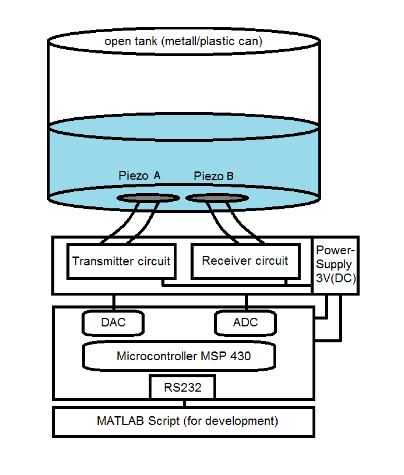
\includegraphics[width=0.35\textwidth]{Chapters/2CHP/Diagrams/stimPiezo.eps}
    \caption{Stimulation and measuring system based on piezo transducer}{\cite{jahnLevelSensorFluids2014a}}
    \label{fig:stimPiezo}
\end{figure}
Another method to produce vibration in the LPG bottle, can be archived with a hammer or a device, that hits the surface of the LPG bottle, the captured signal is the appropriated sensor is then processed and the result returns the level of liquid gas inside. In this case, not only vibration in the bottle is produced but a sound as well\cite{wuAnalysisImplementationNoncontact2016a}.
\begin{figure}[!htb]
    \centering
    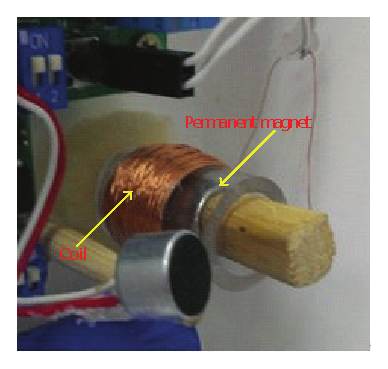
\includegraphics[width=0.45\textwidth]{Chapters/2CHP/Diagrams/stimHammer.eps}
    \caption{Stimulation system based on a knocking device}{\cite{wuAnalysisImplementationNoncontact2016a}}
    \label{fig:stimHammer}
\end{figure}

%----------------------------------------Section 3-----------------------------------

\section{Signals and System}\label{sec:sigNsys}
\subsection{Vibration}
The vibration and the studies in this field are usually related with the oscillatory motion of a body and the forces associated with them. Bodies with mass and elasticity are capable of experience vibration, knowing that, for example, when a structure is design, is required to take in consideration the oscillatory behavior of the structure. There are two types of vibration, free and forced. The first takes place when a system oscillates under forces natural to the system itself and there is no action of external forces. Under free vibration the system will vibrate at one or more of its natural frequencies, stablished by the properties of the system. Forced vibration occurs when the system is under the excitation of external forces. If it oscillatory, the system will vibrate at the same frequency of the external oscillation, if this frequency matches one of its natural frequencies a resonant state is reached, which may dangerous for a structure stability.   

\subsection{Signal definition}
Signals can describe a large variety of physical phenomenon's, bringing a certain information about it, depending of the phenomenon represented. For example, the voltage variation in a capacitor, or the human voice which creates variations in acoustic pressure, captured by a microphone that senses those variations and convert them into a electrical signal. A signal can be represented mathematically as a function of one or more independent variables. 
To what concern in signal processing, the types of signal considered are two types, continuous-time signals and discrete-time signals. In these cases, the independent variable is continuous and discrete, respectively\cite{oppenheimSignalsSystems1997}.

\subsection{Signal and Digitalization}
A continuous-time signal can be represented in a discrete-time form by the knowledge of its values at certain points in time equally spaced. This is called sampling theorem, and if the samples are close to each other, less time between samples, the more similar the discrete signal became to the continuous. Sampling plays an important role between the continuous-time and the discrete-time.

Considering a continuous-time signal $x(t)$ is measured at every $T_{s}$ seconds. The is discretized in units of the sampling interval $T_{s}$:
\begin{figure}[!htb]
    \centering
    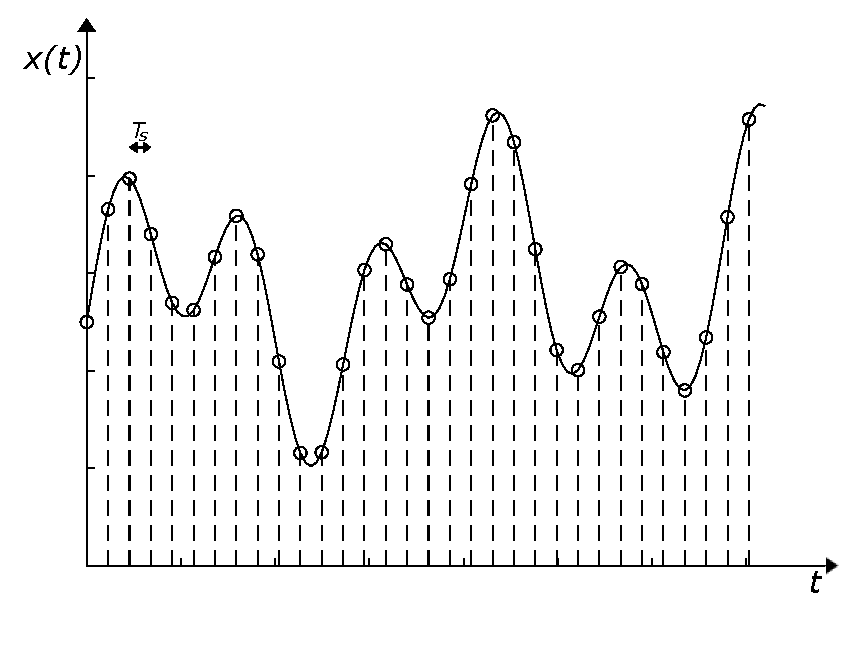
\includegraphics[width=0.45\textwidth]{Chapters/2CHP/Diagrams/sampsignal.eps}
    \caption{Signal sampling}{}
    \label{fig:signalsamp}
\end{figure}
\begin{center}
    $t = nT_s,\> n = 0, 1, 2, ...$
\end{center}
The variable $T_s$ is called sampling period and the inverse of the period $f_s=\frac{1}{T_s}$ being the sampling frequency. One of the problems of this conversion is usually related with the correct choose of the sampling period, for that the theorem clearly specifies that the sampling period must be small enough so if there are small variations in the signal, they don't get lost between samples. Therefor the theorem says that the sampling frequency $f_s$ must be chosen to be  at least twice the maximum frequency $f_{max}$. A continuous-time signal $x(t)$ is bandlimited, so its frequency spectrum is limited at maximum frequency $f_{max}$, and no frequencies above that.

\begin{equation} \label{eq:sampFreq}
       f_s \geq 2f_{max}
\end{equation}
\begin{equation} \label{eq:sampPeriod}
    T_s \leq \frac{1}{2f_{max}}
\end{equation}

The minimum value of the sampling frequency allowed by the theorem, is called the Nyquist rate, and his value is $f_s = 2f_{max}$. Oppositely, for a known value of $f_s$ the maximum frequency of the signal is $f_{max}=\frac{f_s}{2}$ and is called the Nyquist frequency of folding frequency.

For the representation of some signals is usually used a unit impulse as a method to build a block to represent and construct other signals. The simplest representation of a unit impulse (or unit sample), in discrete-time, is defined as follows:
\begin{equation}
    \delta(n) = \left\{ \begin{matrix} 
    0, n \ne 0\\
    1, n = 0\\
    \end{matrix}\right.
\end{equation}
Another example of a simple discrete-time signal is the unit step, defined as:
\begin{equation}
    u(n) = \left\{ \begin{matrix} 
    0, n < 0\\
    1, n \geq 0\\
    \end{matrix}\right.
\end{equation}
If a close analysis is made, is possible to conclude that there is a relation between a unit impulse and a unit step, a unit step can be represented as a sum of impulses
\begin{equation}\label{eq:step}
    u(n) = \sum_{k=0}^{\infty}\delta(n-k)
\end{equation}
The equation \ref{eq:step} can be seen as a sum of delayed impulses and plays an important role in the sampling property.\\
The values of the $f_{max}$ and $f_s$ depend on the application, and the Nyquist frequency usually defines the cutoff frequencies used in filters required in DSP applications. A example of the of the typical sampling rates of common DSP applications are shown in the following table:   
\begin{table}[!htpb]
   \centering
   \begin{tabular}{|c|c|c|} \toprule
       {application}&{$f_max$}&{$f_s$}\\
       \toprule
       {geophysical}&{500 Hz}&{1 kHz}\\
       {biomedical}&{1 kHz}&{2 kHz}\\
       {mechanical}&{2 kHz}&{4 kHz}\\
       {speech}&{4 kHz}&{8 kHz}\\
       {audio}&{20 kHz}&{40 kHz}\\
       {video}&{4 MHz}&{8MHz}\\
       \bottomrule
   \end{tabular} 
   \caption{Common sampling rates per application}{\cite{orfanidisIntroductionSignalProcessing1996}}  
    \label{tab:sampRat}     
\end{table} 

\subsection{System definition}\label{subsec:SysDef}
There is no specific nature to a system, and there is vast example of systems all around us, they could be biological, mechanical, electrical, among others. In the signal processing context a system can be viewed as a process in which input signals are transformed by the system or cause the system to respond in some way, with the resulting in new output signals. Simplifying, a system can be described as an entity with a specific function, where the output signal is the result of the manipulation one or more input signals.
To the types of signals mentioned, continuous and discrete, the systems usually are represented as in the equation \ref{eq:systemeq}, in both cases $x$ represents input and $y$ output.
\begin{figure}[!htb]
    \centering
    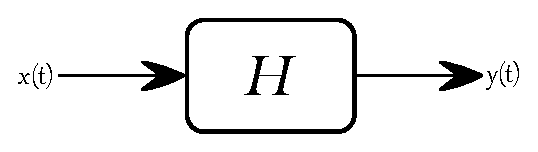
\includegraphics[width=0.45\textwidth]{Chapters/2CHP/Diagrams/systemIll.eps}
    \caption{Generic system}{}    
    \label{fig:piezoresistiveacc}
\end{figure}
\begin{equation} \label{eq:systemeq}
    \begin{split}
        y(t) = H[x(t)] \\
        y(n) = H[x(n)]
    \end{split}
\end{equation}

One of the motivations for the study/analysis of systems from various applications, thus systems from different applications, with similar behavior, can have similar mathematical descriptions. The description of a system as a mathematical function also allows to simulate the behavior in a certain application, testing the response of it with different techniques. 

A system can be described with certain properties, each one having a different effect on the system output. The properties are stability, memory, causality, invertibility, time-invariance and linearity. In signal-processing context, invertibility and time-invariance have special relevance, with a profound study of linear time-invariant(LTI) systems further ahead\cite{oppenheimSignalsSystems1997}\cite{haykin1999signals}.
\subsubsection*{Stability}
A system is considered stable if an input signal limited in amplitude, results in a output signal also limited in amplitude. The system operation, H, is stable if the output signal $y(t)$  satisfies the following condition
\begin{equation}
    |y(t)|\leq M_y < \infty , \forall t
\end{equation}
If the input signal $x(t)$ satisfies the condition
\begin{equation}
    |x(t)|\leq M_x < \infty , \forall t
\end{equation}
The values of $M_x$ and $M_y$ correspond to finite positive numbers. The conditions for the stability of a discrete-time system can be described in the same way.
\subsubsection*{Memory}
A system has memory, when the output signal depends on past values of the input signal. The temporal extension of the past values on which the output depends, defines how far the memory of the system extends. One example of a system with memory is the current $i(t)$ in a inductor and the relation of his voltage $v(t)$:
\begin{equation}
    i(t)=\frac{1}{L}\int_{-\infty}{t}v(\tau)d\tau
\end{equation}
For a discrete-time system, the conditions are similar. 
\subsubsection*{Causality}
A system is considered \textit{causal} if his resulting output signal, only depends in present/past values of the input signal. Opposed to that, a \textit{noncausal} system can have is output depending on future values of the input signal.
An example of a \textit{causal} output is the following:
\begin{equation}
    y(n) = \frac{1}{3}(x(n)+x(n-1)+x(n-2))
\end{equation}
On the other hand an example of a \textit{noncausal} is:
\begin{equation}
    y(n) = \frac{1}{3}(x(n+1)+x(n)+x(n-1))
\end{equation}
\subsubsection*{Invertibility}
A system is considered invertible if is possible to recover the input from the output signal of the system. The operation to recover the signal may be a different system connected to the output of the first. If the operation of a system is represented with $H$ in a continuous-time domain, with $x(t)$ and $y(t)$ being the input and output, respectively. The $y(t)$ is applied to the second system, where the result is expected to be $x(t)$, as follows:
\begin{equation}
    \begin{aligned}
        H^{-1}{y(t)} = H^{-1}{H\{x(t)\}}\\
        = H^{-1}H\{x(t)\}    
    \end{aligned}
\end{equation} 
As the $H^{-1}H$ denotes the identity operation. If $H^{-1}$ is the inverse operation of the $H$ then the output of the second operation is the same as the input of the first operation. This property has special relevance in the design of communications systems. 

\subsubsection*{Time-Invariance}
A system is considered time invariant if a time delay in the input signal, results as well in a delay of the output signal. This means that a certain system will respond in the same way, whenever a signal is applied in input, meaning that the characteristics of the system won't change with time. Considering a continuous-time system, with $x(t)$ and $y(t)$ being the input and the output, respectively. Represented as follows:
\begin{equation}
    y(t) = H\{x(t)\}
\end{equation} 
If the input signal is delayed by $t_0$ seconds, the new input signal is $x(t-t_0)$ and an be described as follows:
\begin{equation}
    x(t-t_0) = S^{t_0}\{x(t)\}
\end{equation}
Where the $S^{t_0}$ represents the delay. So the new output signal $y_i(t)$, resulting from the delay applied in the will be:
\begin{equation}
    \begin{aligned}
        y_i(t) = H\{x(t-t_0)\}\\
        = H\{S^{t_0}\{x(t)\}\}\\
        =HS^{t_0}\{x(t)\}    
    \end{aligned}
\end{equation}
Now considering $y_o$ the output signal of the original system delayed by $t_0$ seconds: 
\begin{equation}
    \begin{aligned}
        y_i(t) = S^{t_0}\{y(t)\}\\
        = S^{t_0}\{H\{x(t)\}\}\\
        =S^{t_0}H\{x(t)\}    
    \end{aligned}
\end{equation}
The system is time invariant if the outputs are equal for an identical input signal $x(t)$. 
\begin{equation}
    HS^{t_0} = S^{t_0}H
\end{equation}
This means that, for a system $H$ to be time invariant, the system $H$ and the time delay $S^{t_0}$ must commute with each other for $t_0$. A similar relation in the discrete-time system to be time invariant.  
\subsubsection*{Linearity}
A system is considered \textit{linear} if fills all the requirements of the \textit{principle of superposition}. That is, if the response of a system to a weighted sum of input signals is equal to the same weighted sum of the output signals, in each one of the output signals being the result of a certain input signal acting independently in the system. If this principle is not fulfilled, the system is called \textit{nonlinear}. 
A weighted sum of continuous-time signals: 
\begin{equation}
    x(t) = \sum_{i=1}^{N}a_ix_i(t)
\end{equation}
Is applied to a system $H$, where $a_1, a_2, ..., a_N$ correspond the weight factor and $x_1(t), x_2(t), ..., x_N(t)$ correspond to the input signals. Resulting in the system response as represented:
\begin{equation}
    \begin{aligned}
        y(t) = H\{x(t)\}\\
        =H\Bigg\{\sum_{i=1}^{N}a_ix_i(t)\Bigg\}\\
    \end{aligned}
\end{equation} 
If the system is linear then, the weighted sum of output signals is:
\begin{equation}
    \begin{aligned}
        y(t) = \sum_{i=1}^{N}a_i y_i(t)\\
        y_i(t) = H\{x_i(t)\}   
    \end{aligned}
\end{equation}
This result in
\begin{equation}
    y(t) = \sum_{i=1}^{N}a_i H\{x_i(t)\}    
\end{equation}
which is the equivalent mathematical representation as in a weighted sum of inputs. To represent them in the same form, the system operation can commute with the amplitude and sum scaling. This principle also applies to discrete-time systems in a similar form. 


\subsection{LTI Systems} \label{subsec:LTI}
As systems can be found all around us, so does a LPG bottle can be considered as a system. If the mathematical model that represents it meet the last two properties mentioned, it can be referred as a linear time-invariance (LTI) system. These properties combined with the characteristics of the unit impulse, being able to represent common signals as a representation of combined delayed impulses, this allows to completely characterize a LTI to what referrers his impulse response\cite{oppenheimSignalsSystems1997}\cite{haykin1999signals}.
Similar to a unit step $u(n)$, a common signal $x(n)$ can be represented by unit impulses, as follows:
\begin{equation}
    x(n) = \sum_{k=-\infty}^{+\infty} x(k)\delta(n-k)
\end{equation}
In this case the weights in the linear combination are $x(k)$. Another aspect to take in consideration in these types of systems, is the response of the system to a impulse $\delta(n)$, results in $h(n) = H[\delta(n)]$. With this in mind, the response of a linear system $y(n)$ to a common input signal $x(n)$, represented from a combination of shifted impulse, can be represented as:
\begin{equation}
    \begin{matrix}
        y(n) & = & H\big[x(n)\big] \\
        \ & = & \sum_{k=-\infty}^{+\infty} x(k)h(n-k)
    \end{matrix}
\end{equation}
The result is known as the \textit{convolution sum} or \textit{superposition sum} and the operation as \textit{convolution} of the sequences $x(n)$ and $h(n)$. The operation can be represented as:
\begin{equation}
    y(n) = x(n) * h(n)
\end{equation} 
\subsection{Discrete-Time Fourier-Transform}
For the analysis of LTI systems, one of the most powerful and used tools is the Fourier-Series and Fourier Transform. For the analysis purpose, the focus is only going to be the Discrete-Time Fourier-Transform (DTFT). The study of this type of systems offers two great advantages:
\begin{itemize}
    \item It is possible to construct a extensive and convenient class of signals, based on a set of simpler signals.
    \item The response of the LTI signal should be simple enough, to provide a convenient representation of the response from the system to any signal based on the combination of several other basic signals. 
\end{itemize} 
The properties are provided by a set of exponential signals, this is important because the response of a LTI system to a complex exponential input, is the same exponential with the change in amplitude. When dealing with complex exponential signals, for the domain of analysis changes, which is in this case the frequency domain. \\
For the analysis purpose, is necessary to know the representation of a signal $x(n)$, that later is going to be represented as a input of a system. The signal is represented in the frequency domain, where $\omega$ represents the \textit{angular frequency}, and its period is $2\pi$. The signal is represented as follows:
\begin{equation}
    X(e^{\jmath \omega})=\sum_{n=-\infty}^{+\infty}x(n)e^{-\jmath \omega n}
\end{equation}
As mentioned in \ref{subsec:LTI}, the response of a LTI system to a impulse, can be represented by the \textit{convolution} operation. This operation can be represented in the frequency domain as:
\begin{equation}
    Y(e^{\jmath\omega})= X(e^{\jmath\omega})H(e^{\jmath\omega})
\end{equation}
Where the terms $X(e^{\jmath\omega})$, $H(e^{\jmath\omega})$ and $Y(e^{\jmath\omega})$ are the Fourier transforms of $x(n)$, $h(n)$ and $y(n)$, respectively. The \textit{convolution} operation in the LTI system, is easily represented using the Fourier transform with a simple algebraic operation, by multiplying the Fourier transforms. This facilitates the analysis of the signals and systems and increases the understanding in the behavior of the LTI system when a signal is applied to its input.\\

With this work in consideration, a algorithm was presented by Cooley and Tukey, the fast Fourier Transform, or simply FFT. This algorithm later proved to be suitable for a digital implementation, with its reducing time in computing the transforms by order of magnitude\cite{oppenheimSignalsSystems1997}.



% ---------------------------------------Section 4-------------------------------------------------
\section{LPG cylinder Model}\label{sec:LPGModel}
As already mentioned \ref{subsec:SysDef}, is possible to describe an LPG cylinder over a mathematical function, as a system. Being, in many cases, the description similar to other systems. The fact that the system is described as a mathematical model allows to understand what it could be the behavior of it. 

The work developed by \citeauthor{wuLiquidLevelDetector2014b} proposes a model for the LPG cylinder, based on acoustic principals to perform measurements. The procedure that they implement is quite simple, by knocking on the side of the cylinder, that generates the sound, usually that sound changes according to the amount of liquid inside of the cylinder, to evaluate what is the amount of gas inside, the vibration in the cylinder wall is recorded and the frequency of the sound give is proportional to the amount of gas present inside.

Before them, other researches were conducted to study the transverse vibration of cylindrical tubes with variable levels of liquid inside. One of them is the work of \citeauthor{chanFreeVibrationCantilever1995} who proposed a vibration model (clamped-free model), where a tube, clamped at bottom and free at top, was used to study the relations resonant frequencies versus liquid levels. Their tests were conducted under a controlled environment, for different levels of liquid, and the experimental results obtained were in accordance with the theoretical calculations\cite{chanFreeVibrationCantilever1995}. 
Their work was then extended with a different approach by \citeauthor{chanFREEVIBRATIONSIMPLY1996}, the model they proposed study the vibration of a simply supported beam with uniform mass, partially loaded, in one of the sides, with a distributed mass(pinned-pinned model). For the conducted tests, the load length added increases until reaching the the length of the beam, the results obtained in their measurements agreed with the results obtained from the previous work\cite{chanFREEVIBRATIONSIMPLY1996}. 
A few years later \citeauthor{jacobsContactlessLiquidDetection2005} proposed a similar model to \citeauthor{chanFreeVibrationCantilever1995} model, but this time with different boundaries, clamped at bottom and top (clamped-clamped model). The tests conducted measure the resonant frequency of the tube, for different levels of liquid, and their results fitted with the results obtained in the previous mentioned tests\cite{jacobsContactlessLiquidDetection2005}.
Like in the previous studies, the base of the work developed by \citeauthor{wuLiquidLevelDetector2014b} is the Euler-Bernoulli beam theory\cite{raoMechanicalVibrations2017}\cite{thomsonTheoryVibrationApplications1996}, this is used to create a model of a cylindrical tube, allowing to estimate the vibration frequencies for different liquid levels. In their work they were able to prove that this theory can be applied to the vibrations in a LPG cylinder, where the results obtain similar to the results obtained in previous works, also based in the same principal.

\subsection{Mathematical Model for LPG cylinder}
The similarities with the Euler-Bernoulli theory and its models, with a LPG cylinder, is related with the construction of the cylinder. A common LPG cylinder used in house appliances has two welded seams, located at the bottom and the top, and those seams are considered the boundaries of the LPG. These boundaries are not considered to be free, but loose instead, with doesn't allow to immediately conclude which type of the mentioned boundaries the cylinder has. Before getting into a conclusion is necessary to understand the theory behind their work.

If a hammer is used to knock the lateral surface of the LPG cylinder, this will trigger a transverse vibration, considered in this case a mechanical vibration. This vibration is similar to Euler-Bernoulli beam, assuming a distributed mass per unit of length $m$, partially loaded with a distributed mass as well $m_d$, corresponding in this situation to the liquid part of the cylinder. In \ref{fig:mechanicalmodel} is identified the boundaries and is illustrated the LPG cylinder model, the  equation \ref{eq:beamEqSimp} describe the vibratory model of the LPG cylinder. The liquid-gas interface corresponds to the origin, and $EI$ is a constant value corresponding to the the beam flexural rigidity
%Mechanical model of the LPG bottle
\begin{figure}[!htb]
    \centering
    \includegraphics[width=0.45\textwidth]{Chapters/2CHP/Diagrams/mathmodelLPG.pdf}
    \caption{The LPG cylinder filled with liquid, with the mechanical representation of the Euler-Bernoulli beam}{\cite{wuLiquidLevelDetector2014b}}
    \label{fig:mechanicalmodel}
\end{figure}
\begin{equation} \label{eq:beamEqSimp}
    \begin{split}
        EI\frac{\partial^4y_1}{\partial x^4} + (m + m_d)\frac{\partial^2y_1}{\partial t^2} = 0,\> & \text{for $-l_w \leq x < 0$} \\
        EI\frac{\partial^4y_2}{\partial x^4} + m\frac{\partial^2y_2}{\partial t^2} = 0,\> & \text{for $0 < x < L-l_w$}
    \end{split}
\end{equation}

The variables $y_1$ and $y_2$ correspond to the transverse vibratory displacements o f the beam. Considering that the seam welding's are not ideally clamped or pinned, and the main transverse vibration is restricted between the two boundaries, is assumed that they have small displacements, that will show flexural vibration. This way their model assumes that there is strong linear springs and torsional springs connected at the boundaries. Which obligates to the boundaries conditions to be formulated taking in consideration these factors, where $k_{S1}$, $k_{T1}$ are the linear and torsional springs constants for the lower welding, and $k_{S2}$, $k_{T2}$ are the correspondent spring constants in the upper welding.
\begin{equation} \label{eq:beamEqEv}
    \begin{split}
        At\>x=-l_w \Rightarrow \begin{cases}
            EI\frac{\partial^2y_1}{\partial x^2} = -k_{T1}\frac{\partial y_1(-l_w,t)}{\partial x}\\
            EI\frac{\partial^3y_1(-l_w,t)}{\partial x^3}=-k_{S1}.y_1    
        \end{cases}\\
        At\>x=L-l_w \Rightarrow \begin{cases}
            EI\frac{\partial^2y_2}{\partial x^2} = -k_{T2}\frac{\partial y_2(L-l_w,t)}{\partial x}\\
            EI\frac{\partial^3y_2(L-l_w,t)}{\partial x^3}=-k_{S2}.y_2    
        \end{cases}    
    \end{split}
\end{equation}

At the bottom a circular steel plate is attached to make the cylinder more stable in relation with the ground, this turns it more stable the the upper part, which allow them to conclude that the value of the constants, linear and torsional springs, of the bottom is higher when compared with the upper values, i.e. $k_{S1}>k_{S2}$ and $k_{T1}>k_{T2}$. The continuity and equilibrium condition at the interface of the liquid, inside the cylinder, are:
\begin{equation} \label{eq:beamEqEquilCond}
    \begin{split}
        y_1(0,t) = y_2(0,t),\> y'_1(0,t) = y'_2(0,t) \\
        y''_1(0,t) = y''_2(0,t),\> y'''_1(0,t) = y'''_2(0,t)
    \end{split}
\end{equation}
This conditions allow them to investigate the relation of the normalized frequency ratio $f_r=f/f_0$, considering $f_0$ as the maximum frequency when there is no liquid inside, and the length ratio $l_w/L$ in their experiments.

\subsection{Relation with previous studies}
So far the model presented show very general boundaries conditions, by controlling the variables, the model can be easily compared with the mentioned model. Taking that into consideration, a demonstration of this similarities was presented and is the following.
    \subsubsection{Clamped-free boundaries}
    For this condition, the values of the variables are considered to be $k_{S1}=k_{T1}\approx\infty$ and $k_{S2}=k_{T2}=0$. When \citeauthor{chanFreeVibrationCantilever1995} proposed this model to calculate the frequencies of a cantilever tube, partially filled with liquid mercury, the cantilever was clamped at the bottom and free at the top, and the transverse vibration was generated by using a hammer to knock the tube\ref{fig:clampedfreemodel}. 
    %clamped-free model
    \begin{figure}[!htb]
        \centering
        \includegraphics[width=0.45\textwidth]{Chapters/2CHP/Diagrams/clampedfreemodel.pdf}
        \caption{Clamped-Free Model}{\cite{chanFreeVibrationCantilever1995}}
        \label{fig:clampedfreemodel}
    \end{figure}
    If the values of the variables are replaced in the equation\ref{eq:beamEqSimp} the result of this setup makes the boundaries conditions at their limits, $x=-l_w$ and $x=L-l_w$, to be as shown in \ref{eq:beamEqClamFree}, when comparing the results in the boundaries conditions they verify that they were the same as in \cite{chanFreeVibrationCantilever1995}.
    \begin{equation} \label{eq:beamEqClamFree}
            y_1(-l_w,t) = y'_1(-l_w,t) = y''_2(L-l_w,t) = y'''_2(L-l_w,t)=0
    \end{equation}
    \subsubsection{Pinned-pinned boundaries}
    For this condition, the value of the variables considered is $k_{S1}=k_{S2}\approx\infty$ and $k_{T1}=k_{T2}=0$. In this model, proposed by \citeauthor{chanFREEVIBRATIONSIMPLY1996}, the study is made in a simply supported beam partially load, with distributed mass in both cases\ref{fig:pinnedpinnedmodel}.
    %Pinned-Pinned Model
    \begin{figure}[!htb]
        \centering
        \includegraphics[width=0.45\textwidth]{Chapters/2CHP/Diagrams/pinnedpinnedmodel.pdf}
        \caption{Pinned-Pinned Model}{\cite{chanFREEVIBRATIONSIMPLY1996}}
        \label{fig:pinnedpinnedmodel}
    \end{figure}
    Once again, if the variables in \ref{eq:beamEqSimp} are replaced with $k_{S1}$, $k_{T1}$, $k_{S2}$ and $k_{T2}$, the result in this setup will also match the boundaries condition\ref{eq:beamEqPinnedx2} at $x=-l_w$ and $x=L-l_w$, obtained in \cite{chanFREEVIBRATIONSIMPLY1996}.
    \begin{equation} \label{eq:beamEqPinnedx2}
        y_1(-l_w,t) = y''_1(-l_w,t) = y_2(L-l_w,t) = y''_2(L-l_w,t)=0
    \end{equation}
    \subsubsection{Clamped-clamped boundaries}
    In this case, the value considered to the variables was $k_{S1}=k_{T1}=k_{S2}=k_{T2}\approx\infty$. This model, proposed by \citeauthor{jacobsContactlessLiquidDetection2005}, with a contactless method to measure the vibration of a opaque capillary tube\ref{fig:clampedclampedmodel}.
    %Clamped-Clamped Model
    \begin{figure}[!htb]
        \centering
        \includegraphics[width=0.45\textwidth]{Chapters/2CHP/Diagrams/clampedclampedmodel1.pdf}
        \caption{Clamped-Clamped Model}{\cite{jacobsContactlessLiquidDetection2005}}
        \label{fig:clampedclampedmodel}
    \end{figure}
    Following the same path of the previous two, the variables $k_{S1}$, $k_{T1}$, $k_{S2}$ and $k_{T2}$ were once again replaced in \ref{eq:beamEqSimp},and the results obtained\ref{eq:beamEqClampedx2} at their boundaries conditions matched results obtained in \cite{jacobsContactlessLiquidDetection2005}
    \begin{equation} \label{eq:beamEqClampedx2}
        y_1(-l_w,t) = y'_1(-l_w,t) = y_2(L-l_w,t) = y'_2(L-l_w,t)=0
    \end{equation}

    \subsubsection{Relation of Frequency versus Length}
    As a final comparison, the test between the relation of the frequency with the length of the liquid level was executed. For that, different values were attributed to linear and torsional spring variables, to allow the simulation of theoretical curves of the normalized frequency ratio $f_r (f_i/f_0)$ and length ratio $l_r (l_w/L)$. The values for each of the variables were chosen to be large enough to simulate the different boundaries conditions. As expected the results[reference to all images] of \citeauthor{wuLiquidLevelDetector2014b} were very similar with what was previously obtained \cite{chanFreeVibrationCantilever1995}\cite{chanFREEVIBRATIONSIMPLY1996}\cite{jacobsContactlessLiquidDetection2005}, confirming what was mention in the beginning of this section.
    %Theoretical curves
    \begin{figure}[!htb]
        \centering
        \includegraphics[width=0.45\textwidth]{Chapters/2CHP/Diagrams/theoricalcurve.pdf}
        \caption{Frequency VS Weight - Practical curve obtained by \citeauthor{wuLiquidLevelDetector2014b}}
        \label{fig:theoCurves}
    \end{figure}
    In this relation is important to note that, when the cylinder is almost empty $l_r = 0$ the frequency of the vibration is the highest, in the opposite cases, when the cylinder is full $l_r = 1$ then the vibration frequency is archives the minimum value. 
\subsection{Experimental results}\label{subsec:SOAExpRes}
In the tests perform by \citeauthor{wuLiquidLevelDetector2014b}\cite{wuLiquidLevelDetector2014b}, their setup consisted in a hammer knocking in the lateral surface of the cylinder, that produces the transversal vibration, which is captured by a microphone,processed with a FFT algorithm. By continuously releasing gas and measure the produced vibration, and the correspondent frequency they obtained the following relation: 
%Practical curve obtained
\begin{figure}[!htb]
    \centering
    \includegraphics[width=0.45\textwidth]{Chapters/2CHP/Diagrams/weightvsfrequency.pdf}
    \caption{Frequency VS Weight - Practical curve obtained by \citeauthor{wuLiquidLevelDetector2014b}}
    \label{fig:practCurve}
\end{figure}
In the same way of their theoretical simulations, the relation between the vibration frequency and the liquid level(or the length of the liquid) is similar, the highest frequency correspond to the lowest liquid level, and the lowest frequency to the highest liquid level. One thing that is important to refer that is mentioned in their work is, this relation is constant for the different variety of LPG cylinders, but the frequency range of each also varies with the amount of gas that they can store\ref{fig:practCurve}, which means that the device must be adapted to the type of cylinder that is going to be used in. 
%Figures of curves from different bottles
\begin{figure}[ht]
    \centering
    \begin{subfigure}{0.45\textwidth}
        \centering
        \includegraphics[width=\linewidth]{Chapters/2CHP/Diagrams/g1line.pdf}
        \caption{}
        \label{subfig:g1lines}
    \end{subfigure}
    \begin{subfigure}{0.45\textwidth}
        \centering
        \includegraphics[width=\linewidth]{Chapters/2CHP/Diagrams/g2line.pdf}
        \caption{}
        \label{subfig:g2lines}
    \end{subfigure}
    \begin{subfigure}{0.45\textwidth}
        \centering
        \includegraphics[width=\linewidth]{Chapters/2CHP/Diagrams/g3line.pdf}
        \caption{}
        \label{subfig:g3lines}
    \end{subfigure}
    \begin{subfigure}{0.45\textwidth}
        \centering
        \includegraphics[width=\linewidth]{Chapters/2CHP/Diagrams/g4line.pdf}
        \caption{}
        \label{subfig:g4lines}
    \end{subfigure}
    \caption{Different LPG cylinder to used to compare the relation between Frequency and Weight for different models}{\citeauthor{wuLiquidLevelDetector2014b}}
     \label{fig:noise}
 \end{figure}
A couple of years latter this work was followed by \citeauthor{wuAnalysisImplementationNoncontact2016a}\cite{wuAnalysisImplementationNoncontact2016a}, were they developed a prototype with the function of measure the frequency of the vibration, and thus the returning the liquid level of the LPG cylinder. The setup used and the test conditions were very similar the the previous work.

\section{Vibration Sensors}\label{sec:VibSens}
To acquire and measure the vibration, the sensors used must work according to the system mechanical or optical principals of vibration. There is a large variety of sensors that ca be used for that purpose, although there isn't a direct method, or sensor, to measure the vibration, they can be either mechanical or optical. The sensors can be divided in different groups, based on their behavior, they can be active or passive, the type of measurement can be either absolute or relative, and there is also some specific characteristics of the signals that differ from the type of sensor, like the frequency range, signal dynamic and the quality of the data acquired. Finally sensors are also divided in contact and non-contact measurement and subdivided in path/displacement, speed/velocity or acceleration.\\
For contact measurements, sensors related to path/displacement can be potentiometric transmitters or Linear Variable Differential Transmitter (LVDT), to speed/velocity it can be applied the principle of electrodynamics or use a seismometer as a sensor and for acceleration the sensors can be piezoelectric, piezo-resistive, resistive or inductive. In non-contact measurements, path/displacement sensors are eddy current sensors, optical sensors and hall sensors, or can be based on the capacitive principle, for speed/velocity is used a Laser-Doppler vibrometer (LDV) and for acceleration isn't possible to measure directly, although it can be derivate from speed/velocity measurement, but induces a lot of noise in the data acquired\cite{SensorsVibrationMeasurement}\cite{VibrationMeasurementVibration2019}.\\
To measure the vibration, usually is the contact acceleration the most common method to measure them, beside the sensors mentioned, is used as well accelerometers, this devices are used in industry to reliably measure vibration in equipment, to monitoring their health.The functioning  principles of accelerometers can differ from one to another. The basic principle of a accelerometer is similar to a seismometer, from this there are 3 main types, mechanical, capacitive and piezoelectric. The mechanical is the most similar to a seismometer, with a mass attached to a spring, every time that acceleration occurs, just like in seismometer, the mass moves and a pen attached to the mass traces the vibration captured.
\begin{figure}[!htb]
    \centering
    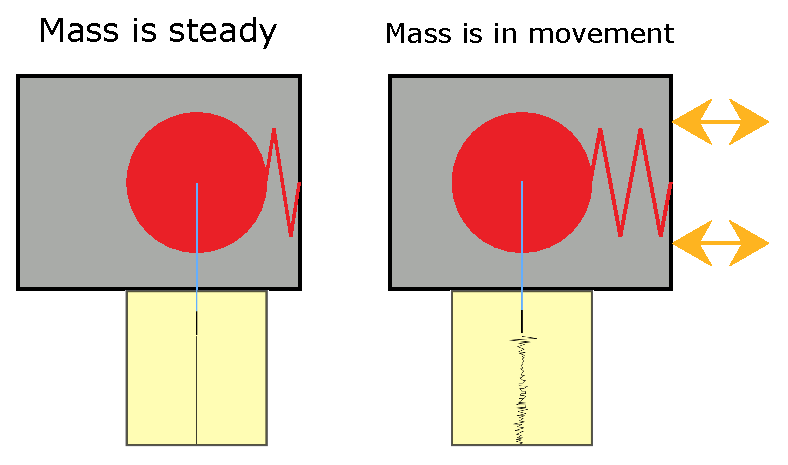
\includegraphics[width=0.45\textwidth]{Chapters/2CHP/Diagrams/seismometer.eps}
    \caption{Illustration of the working principle of simple accelerometer}{}    
    \label{fig:seismometer}
\end{figure}
%%Insert here a image to illustrate this
% see in https://www.explainthatstuff.com/accelerometers.html  
Although in the case of the accelerometer, doesn't trace with a pen in paper, instead generates a electrical or magnetic signal. A example of this, is a piezoresistive accelerometer, which has a his mass attached to a potentiometer, and the result of the vibration is a voltage change. When a magnetic variation occurs, usually a hall-effect accelerometer is used for that effect.  
Similar to the mechanical, a capacitive accelerometer, has one of the plates attached to the mass, and measures the capacitance variation, the vibration of capacitance is related with the vibration movement. 
%% Insert another image here
\begin{figure}[!htb]
    \centering
    \includegraphics[width=0.45\textwidth]{Chapters/2CHP/Diagrams/capacitiveacc.eps}
    \caption{Illustration of the working principle of capacitive accelerometer}{}    
    \label{fig:capacitiveacc}
\end{figure}
In piezoelectric accelerometers, the function principle is similar to the previous, the mass is attached to the piezoelectric and when it moves causes a deformation. The resulting signal from the deformation is the result of the piezoelectric effect. A piezoelectric consist in two metal plates with piezoceramic material between them, usually a quartz crystal. To produce electricity, the piezoceramic material needs to be under stress, that is, to be compressed or squeezed. This caused a voltage different the two metal plates, this is the result of the collection of charges produced in the piezoceramic material.
%%Insert here
\begin{figure}[!htb]
    \centering
    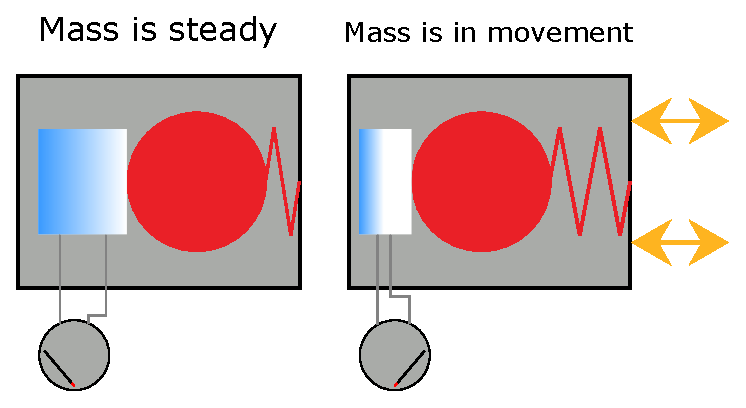
\includegraphics[width=0.45\textwidth]{Chapters/2CHP/Diagrams/piezoresistiveacc.eps}
    \caption{Illustration of the working principle of a piezoresistive accelerometer}{}    
    \label{fig:piezoresistiveacc}
\end{figure}
All the type of accelerometers mentioned have one problem, that is the fact that they aren't practical to use in certain application, as an example a small electronic device. For that, is used the so called MEMS (Micro Electro Mechanical Systems) accelerometers, this type of accelerometer is a combination of electrical and mechanical device, mounted on a silicon chip, this is one advantage of this type of accelerometers, the can be very produced in very small sizes, to allows their application in different types of electronic devices. The functioning of this type of accelerometer can be explained quite easily, an electrode is between two other electrodes, there is a air gap between these two and a small insulation to prevent direct contact between the middle electrode and the other two, on the top and the bottom. The middle electrode is connected with a cantilever, rigid enough to hold his position, but flexible enough to allow the move when the accelerometer moves or tilts, the cantilever is connected to outside of the chip, this is used to measure the difference of capacitance between the middle electrode and the electrodes at the top and at the bottom, the capacitance changes every time the middle electrode moves or tilts.\\
 %%insert the image here as a example, get it from https://www.explainthatstuff.com/accelerometers.html
 \begin{figure}[!htb]
    \centering
    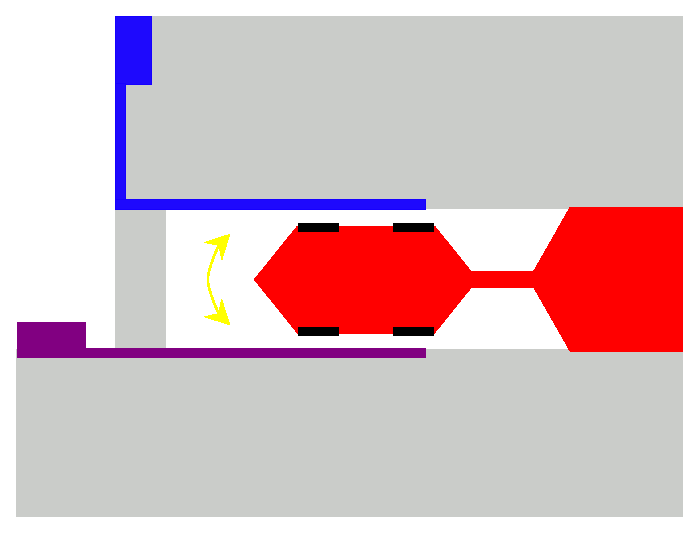
\includegraphics[width=0.45\textwidth]{Chapters/2CHP/Diagrams/memsacc.eps}
    \caption{Illustration of the working principle of a MEMS accelerometer}{}    
    \label{fig:piezoresistiveacc}
\end{figure}
This type of accelerometers brought important advantages, being their low cost and their small size the most important of it. On the other hand, the use of this devices for condition monitoring is restricted to a small bandwidth, restricted to a few kHz, and it cannot be used to in applications that require lower noise over higher frequency ranges \cite{WhatYouNeed}\cite{HowAccelerometersWork2009}.

\clearpage
\printbibliography[heading=subbibliography]
\addcontentsline{toc}{section}{References}

%%%%%%%%%%%%%%%%%%%%%%%%%%%%%%%%%%%%%
% AV1 Video Codec
\cleardoublepage
\chapter{Implementation} \label{chap:trans}
\section{Signal Simulations}
\section{FFT implementation}
\subsection{}
\section{Signal Acquisition} %Change latter
\section{Hardware Developed} %Change latter


% \begin{figure}[!htb]
%     \centering 
%         \begin{subfigure}[c]{\textwidth}
%             \centering
%             \input{Sections/3Transforms/Images/DFTSymmetry.tex}
%             \caption{}
%             \label{subfig:dft}
%         \end{subfigure}
%         \begin{subfigure}[c]{0.45\textwidth}
%             \centering
%             \input{Sections/3Transforms/Images/DCT1Symmetry.tex}
%             \caption{}
%             \label{subfig:dct1}
%         \end{subfigure}
%         \begin{subfigure}[c]{0.45\textwidth}
%             \centering
%             \input{Sections/3Transforms/Images/DCT2Symmetry.tex}
%             \caption{}
%             \label{subfig:dct2}
%         \end{subfigure}
%         \begin{subfigure}[c]{0.45\textwidth}
%             \centering
%             \input{Sections/3Transforms/Images/DCT3Symmetry.tex}
%             \caption{}
%             \label{subfig:dct3}
%         \end{subfigure}
%         \begin{subfigure}[c]{0.45\textwidth}
%             \centering
%             \input{Sections/3Transforms/Images/DCT4Symmetry.tex}
%             \caption{}
%             \label{subfig:dct4}
%         \end{subfigure}
%         \caption{Sequences generated in the first step of Table \ref{tab:DFTDCT}for the DFT and different DCTs. Filled dots correspond to the original sequence ((a) - \emph{DFT}; (b)) - \emph{DCT-I}; (c)) - \emph{DCT-II}; (d)) - \emph{DCT-III}; (e)) - \emph{DCT-IV}).}
%     \label{fig:2NSeq}
% \end{figure}
% \begin{lstlisting}
%     ./aomenc <INPUT-FILE> -h <HEIGHT> -w <WIDTH> -o <OUTPUT-FILE> --limit=10 -p 1 --cpu-used=8 --i420 --q-hist=64 --end-usage=q --cq-level=<CQ-LEVEL>
% \end{lstlisting}
\clearpage
%\printbibliography[heading=subbibliography]
%\addcontentsline{toc}{section}{References}

%%%%%%%%%%%%%%%%%%%%%%%%%%%%%%%%%%%%%
% Developed Architecture
\cleardoublepage
\chapter{Hardware}\label{chap:hardware}
This chapter consists in the identification of the physical components to use in the solution to develop, from the proposed approach. It will be explained the selection of each one of them and their purpose in the system. Beside this will be briefly explain the hardware developed for signal conditioning and to stimulate the system. In the end, will be presented some methods to attach the sensors to the bottle.
\section{Selection}
This section presents the selection process of each sensor and its purpose in the application. What were the criteria to select the sensors to measure the vibration,  to process the data and to stimulate the system. 
\subsection{Microphone}
With the intent of understanding what is the system response to an external stimulation, is necessary a method to record that response. The easiest way to do that is by using a microphone to capture the sound produced, when hitting the side surface of the \acrshort{lpg} bottle.
The choice to use as a microphone was the one embedded in the phone. By the time the study started, was the most practical option available. The phone itself is connected via USB to the computer, on which additional software was installed to allow access in real time to the microphone of the phone.  
\subsection{Accelerometer}
As already mentioned in section \ref{sec:VibSens}, there are various types of accelerometers, however the choice depends on various factors. In this particular application is important that the accelerometer in use has a low cost and a small size, for the future application. With this in mind the choice declines over MEMS accelerometers, which are smaller when compared with piezoelectric accelerometers.

The type of \acrshort{mems} accelerometers available is very wide, some of them started to be used in applications that usually uses piezoelectric accelerometers, like condition-based monitoring, structural health monitoring, asset health monitoring, vital sign monitoring and \acrshort{iot}. When selecting the accelerometer it is important to take into consideration some parameters, which are responsible to determine the category of the accelerometer, their application, the bandwidth and the range. Although there is no standard for the category on each accelerometer fits in, \acrlong{ad} has one document where they divide their products in different categories, with the type of application where each one can be used, featuring a description of the key parameters, that must be taken into consideration when selecting the appropriate accelerometer~\cite{AnalogDialogue51102017}.
\begin{figure}[]
    \centering
    \includegraphics[width=1\textwidth]{Chapters/4CHP/Figures/adTable.pdf}
    \caption{Application landscape for a selection of Analog Devices MEMS accelerometers}
    \label{fig:adtable}
\end{figure}

The \acrshort{mems} accelerometers, from Analog Devices, are divided in two families, the ADXLxxxx and the ADIS16xxxx. The last offers different advantages when compared with the first, especially like a plug-and-play solution with features like factory compensation, embedded compensation and signal processing. This family has one of the features that has particular interest for the application, in this case the fact that it has signal processing on the accelerometer. On the other hand this family of products has a higher cost, which is not ideal if the final solution is suppose to be affordable. So it is necessary to define the key specifications of the accelerometer, in order to properly select one~\cite{AnalogDialogue51102017}.

The final purpose is to have a cheap and portable prototype, that is capable of accurately measuring the vibrations and determining the liquid level. This implies that the bandwidth covers the spectrum of frequency on which the curve of the relation liquid level vs frequency is. With this in mind the key specifications are the low cost, low power and his bandwidth. According to the results obtained by~\citeauthor{wuLiquidLevelDetector2014b}\cite{wuLiquidLevelDetector2014b} shown in section~\ref{sec:LPGModel} and the maximum frequency for a mechanical vibration, shown in table~\ref{tab:sampRat}, it can be used an accelerometer with a Bandwidth close to 2kHz. Considering these specification, some models where chosen, that integrate this criteria, as follows:
\begin{table}
    \centering
    \includegraphics[width=1\textwidth]{Chapters/4CHP/Figures/accTable.pdf}
    \caption{Key specifications of MEMS accelerometers}
    \label{tab:acctable}
\end{table}

Although it does not accommodate entirely the specifications, but since it was already available for use, the choice fell to the ADXL335. This model offers a low power consumption of around 350$\mu$A, its bandwidth is adjustable with a single capacitor per axis, from 0.5 to 1600 Hz for X and Y axis and 0.5 to 550 Hz for Z axis. Beside this the accelerometer itself is very cheap, with a price starting at 3€. To properly acquire the data from this sensor and process it, it is necessary to integrate it with an amplifier circuit and a microcontroller, on which more details will be explained further ahead.
\subsection{Piezoelectric}

There are several types of piezoelectric constituents, a defining factor of the type of material used in the piezoelectric, is his application. The most commonly used in vibration measurement is \acrshort{pvdf} as polymer and \acrshort{pzt} as ceramic. This sensor produces charges according to the applied pressure and the voltage generated at the output is related with the amount of charges generated. In a electric point a view, this is a sensor with a high-impedance, therefore is necessary a amplifier circuit with a high input impedance and with a high \acrshort{snr} relation. For piezoelectric it is usual to use a charge amplifier, that already fills these requirements.

In the developed work, two different piezoelectric were used, with different dimensions, one with a diameter of 27mm and the other with a diameter of 12mm.

\begin{figure}[]
    \centering
    \begin{subfigure}{0.45\textwidth}
        \centering
        \includegraphics[width=\linewidth]{Chapters/4CHP/Figures/piezo27mm.png}
        \caption{}{}
        \label{subfig:piezo1}
    \end{subfigure}
    \begin{subfigure}{0.45\textwidth}
        \centering
        \includegraphics[width=\linewidth]{Chapters/4CHP/Figures/piezo12mm.png}
        \caption{}{}
        \label{subfig:piezo2}
    \end{subfigure}
    \caption{Piezoelectric sensors used}{}
    \label{fig:UsedPiezos}
\end{figure}
The use of a piezoelectric is not only a cheaper option, when compared with the accelerometer, but also, allows to pursue a different approach. This is related to the stimulation technique of the system, that can replace the hitting to a different technique that uses the piezoelectric. 

\subsection{Microcontroller}
When selecting the microcontroller, it is important to have some specifications in mind, as in the perspective of a future implementation. Some are quite quite important, as the performance, the cost, as well as the power consumption. There is a large variety of products that most certainly would fit in these specifications. The selection of this it took in consideration those characteristics and fell to one from \acrlong{ti}. The model of the chosen, is the MSP-EXP430FR2433 and his characteristics are the following:
\begin{itemize}
    \item 16-bit \acrshort{risc} processor with a clock frequency up to 16MHz;
    \item 15KB of program and 512B information \acrshort{fram}, 4KB \acrshort{ram};
    \item 8-channel 10-bit \acrshort{adc};
    \item Four 16-bit Timers, 16-bit counter-only \acrshort{rtc};
    \item 32-bit Hardware-Multiplier;
    \item Two \acrshort{eusci}\_A, supports \acrshort{uart}, \acrshort{irda} and \acrshort{spi} and one \acrshort{eusci}\_B, supports \acrshort{spi} and \acrshort{i2c};
\end{itemize}
Beside these characteristics, the microcontroller offers different low-power modes, that consume from several hundreds of microAmps to a couple of hundreds of microAmps, depending on the mode of operation of the microcontroller. Another thing in consideration, when selecting, is the fact that it is possible to run with a super cap. The performance in this case is not as important as it seems as it is not mandatory that an operation that would need to be performed must return the result to the user instantly, that means that the results not being in real time will not make much of a difference anyway if that was the case. There is also a 32-bit Hardware-Multiplier embedded, that reduces the use of \acrshort{cpu} time to perform multiplications that would be required\cite{MSP430FR2433DataSheet}. Associated with these characteristics, the price of this microcontroller is very appealing, starting under 2€.

\subsection{Solenoid}
Since the use of the hammer to hit the bottle is not practical and has inconstant results, a solenoid will be used with the intention of substitute the hammer. This way, is possible to stimulate the system automatically by powering the solenoid. With that purpose the SOL01002 was selected because this solenoid works with voltages starting at 5V and the other reason is due the fact that is a Push type, which means that when powered the shaft will move and produce the desired impulse.
\begin{figure}[]
    \centering
    \includegraphics[width=0.45\textwidth]{Chapters/4CHP/Figures/solenoide.jpg}
    \caption{Solenoid used to stimulate the bottle}
    \label{fig:solenoid}
\end{figure}
The downside of using this model, can be the low impact force, it may not be able to produce a strong enough hit detectable by the sensors.
\section{Design}
This section is dedicated to explain how each circuit was planned to interact with the sensors in use, being important to the design what is the output of each signal. Before getting into details of each circuit, the resulting signal of each sensor and the consideration to further design the circuit will be presented.

\subsection{Accelerometer}
Considering that the accelerometer has three outputs, that are limited in frequency with a capacitor, the output used was the X axis with a bandwidth of 1600Hz, which is the maximum frequency.
\begin{figure}[]
    \centering
    \includegraphics[width=0.45\textwidth]{Chapters/4CHP/Figures/accTopView.pdf}
    \caption{Top view of ADXL335}
    \label{fig:topViewADXL}
\end{figure}

Considering the dot shown in the top view of the ADXL335, in figure~\ref{fig:topViewADXL}, when mounting the accelerometer in the side surface of the \acrshort{lpg} bottle, the dot is in the same position relative to the surface, on the top left corner. This way the output of the X axis measured, is around 1.25V, if the accelerometer is powered with 3.3V. Before designing the circuit to amplify the signal from the accelerometer is important to know, what should be the gain of the circuit. For that the surface of the bottle was hit with the hammer and the resulting output can be observed in figure~\ref{subfig:maxAccNDC}, approximately at the center of the image. In figure~\ref{subfig:maxAccN} is the same signal with zoom.

\begin{figure}[]
    \centering
    \begin{subfigure}{0.45\textwidth}
        \centering
        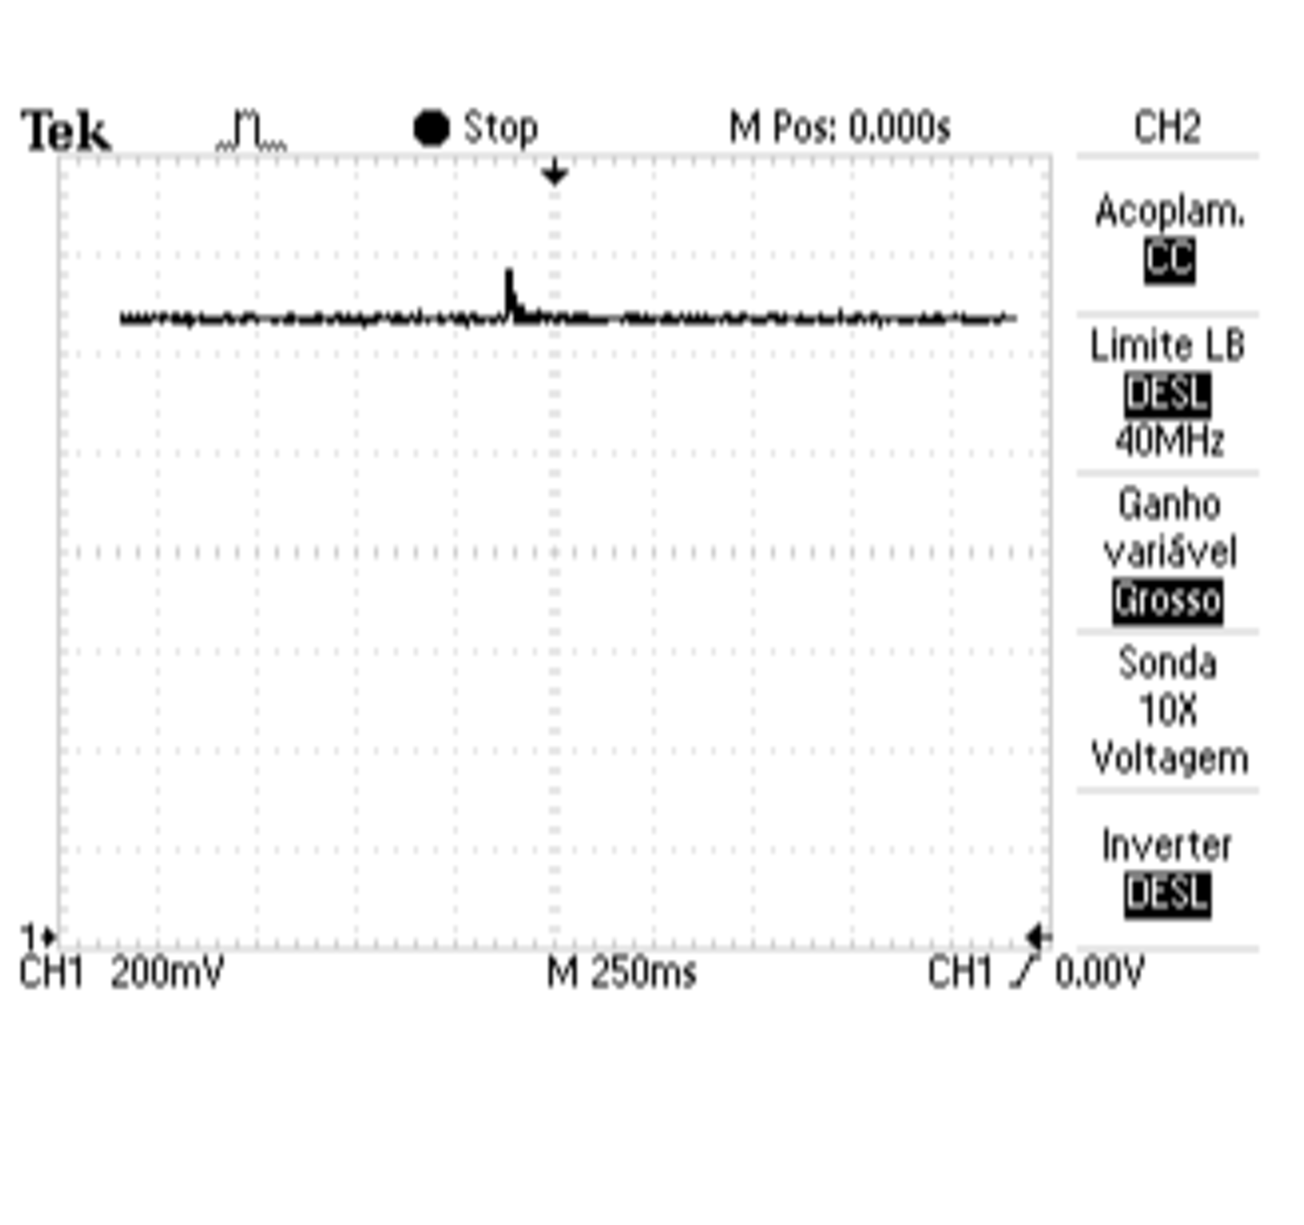
\includegraphics[width=\linewidth]{Chapters/4CHP/Figures/maxAccNDC.eps}
        \caption{Signal obtained after hitting in DC level}{}
        \label{subfig:maxAccNDC}
    \end{subfigure}
    \begin{subfigure}{0.45\textwidth}
        \centering
        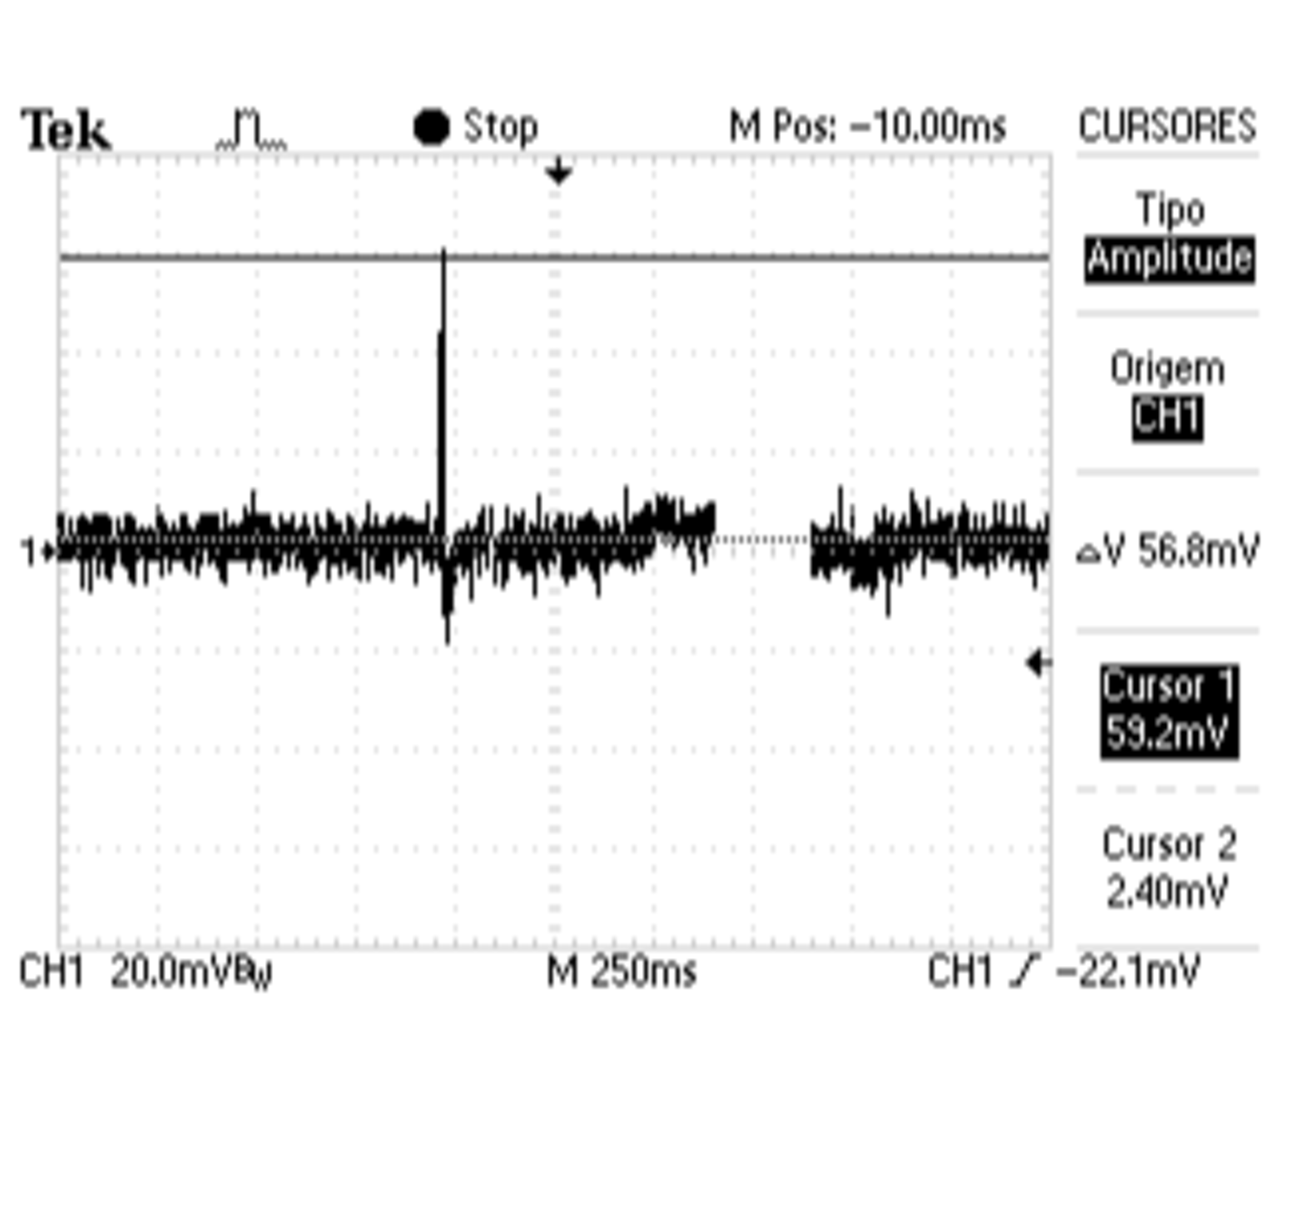
\includegraphics[width=\linewidth]{Chapters/4CHP/Figures/maxAccN.eps}
        \caption{Signal obtained after hitting, in AC}{}
        \label{subfig:maxAccN}
    \end{subfigure}
    \caption{Signal obtained in the accelerometer after hitting with the hammer}
    \label{fig:NampSigAcc}
\end{figure}

Considering that the output of the amplified signal should be between the supply voltage range, that is from 0-3.3V, being the minimum of the signal corresponding to one of the limits of the interval and the maximum to the other. If the amplifier circuit has an inverting configuration, the relation between the input and the output should be as illustrated in figure \ref{fig:inVSout}.
\begin{figure}[]
    \centering
    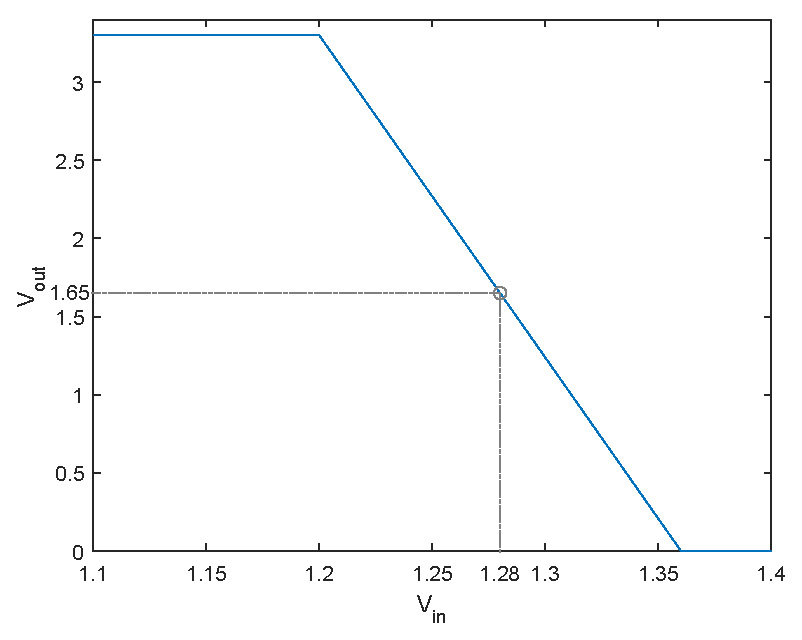
\includegraphics[width=0.45\textwidth]{Chapters/4CHP/Figures/inOut.eps}
    \caption{Desire relation between input and output of the amplifier circuit}
    \label{fig:inVSout}
\end{figure}

The gain of the circuit is determined in the following method:
\begin{equation}
   m = |\frac{\delta V_{Out}}{\delta V_{In}}| \approx |\frac{0-3.3}{1.3-1.2}| \approx 33
\end{equation}

In the equation, $m$ corresponds to the gain of the circuit, in this case only concerns is, the manual stimulation of the system. When changing to a automatic stimulation, is probable that the gain needs to be adjusted, considering the same procedure.

%%
A problem when design a proper circuit for this application is related with his supply voltage. Usually a amplifier circuit with an \acrshort{opamp}, the supply voltage is split, which means that the input/output signals are referenced to the ground. Since it will be used a battery or a super cap to power the device, limits us to a single supply.

In these situations, depending on the circuit configuration, the circuit may not operate for a determinate input voltage, since both input and output are referenced to the ground, thus the circuit will not function properly. In a dual supply voltage, if the supply voltages are symmetrical, the circuit is referenced to his midpoint, which is the ground. In a single supply it can be done in the same way, the signal can be referenced to half of the supply voltage, this is the simplest way to solve the presented problem. 

For now, to prove the concept, the circuit in use can be solved in the simplest way. In some situations and in a future application it may be needed to develop a robust solution for this. For those situations \acrshort{ti} provides a document that explains all the considerations that need to be taken into account and how to properly design the circuit for our application~\cite{manciniSingleSupplyOpAmp}.

As mentioned, to quickly test, is considered an inverting configuration is used to the amplifier circuit and the signal is referenced to the midpoint of the single supply voltage of the \acrshort{opamp}. As for the input signal, a capacitor is used in series to decouple from the DC level, this way the signal is "moved" to the midpoint between the supply voltage as referenced in the design from \acrshort{ti} in their document, providing a schematic for both non-inverting and inverting configuration~\cite{ACCoupledSingle2015}.

Figure~\ref{fig:accCircCom} shows the circuit used to amplify the signal from the accelerometer. Although the output of the accelerometer is around 1.25V, using the decoupling capacitor we are able to move the signal to the midpoint of the supply voltage. The only thing necessary is to adjust the gain of the circuit according to the desire relation between the input and output signals.
\begin{figure}[]
    \centering
    \begin{subfigure}{0.3\textwidth}
        \centering
        \includegraphics[width=\linewidth]{Chapters/4CHP/Figures/AmpAccCirc.pdf}
        \caption{}{}
        \label{subfig:AccAmpCirc}
    \end{subfigure}
    \begin{subfigure}{0.3\textwidth}
        \centering
        \includegraphics[width=\linewidth]{Chapters/4CHP/Figures/HalfSupply.pdf}
        \caption{}{}
        \label{subfig:VoltageDiv}
    \end{subfigure}
    \caption{Amplifiers circuit for accelerometer\ref{subfig:AccAmpCirc} and Midpoint supply voltage~\ref{subfig:VoltageDiv}}{}
\label{fig:accCircCom}
\end{figure}

\subsection{Piezoelectric}
As mentioned, piezoelectric sensors can be used in many fields, for sensing acceleration, vibration, shock or pressure. To what is related to acceleration or vibration, the piezoelectric will output a charge that is a function of his deformation/deflection. For the application in specific, the vibration produce, although is noticeable directly at the piezoelectric output, has a small amplitude which means that needs to be amplified to allow a distinct difference between what is actually the vibration and the output of the piezoelectric itself. To solve this, is important to properly design a signal conditioning amplifier circuit. \acrlong{ti} has a very clear document explaining how to design charge amplifiers for piezoelectric sensors~\cite{bartolomeSignalConditioningPiezoelectric2010}, on which they explain different types of circuits for this application in specific, with the advantages and disadvantages. The simplest model of this type of circuit is as follows~\ref{fig:ChargeAmpSimp}: 
\begin{figure}[]
    \centering
    \includegraphics[width=0.45\textwidth]{Chapters/4CHP/Figures/singleenddedchargeamp.pdf}
    \caption{Charge Amplifier for signal conditioning}
    \label{fig:ChargeAmpSimp}
\end{figure}

Two important things to consider is the bandwidth and the gain of the circuit. In the first case, the circuit functions as a High-Pass Filter which means that when selecting the feedback resistor and capacitance, their values must be selected to keep the cut off frequency low. The equation~\ref{eq:fhpf} can be used to define the cut off frequency.
\begin{equation}\label{eq:fhpf}
    f_{HPF} = \frac{1}{2\pi R_{FB}C_{FB}}
\end{equation}

Usually, the value of the resistor in use is on the order of hundreds of megaohms and the capacitance should be low. The reason is due to the fact that in these circuits the gain is defined by the value of the capacitance, the lower the value, the higher the gain~\ref{eq:gaincharge}.
\begin{equation}\label{eq:gaincharge}
    Gain = \frac{1}{C_{FB}} (mV/C)
\end{equation}

Another factor that must be taken in consideration is the \acrshort{snr}, which needs to be maximized. For this circuit in specific, one way to achieve this is by increasing the value of $R_{FB}$ as much as possible. To outline this and improve the \acrshort{snr} value, a differential charge amplifier is used.

\begin{figure}[]
    \centering
    \includegraphics[width=0.45\textwidth]{Chapters/4CHP/Figures/differentialchargeamp.pdf}
    \caption{Differential Charge Amplifier for signal conditioning}{\cite{bartolomeSignalConditioningPiezoelectric2010}}
    \label{fig:ChargeAmpDif}
\end{figure}

Since this types of circuit are very sensitive to interference, the differential charge amplifier offers one advantage when compared with the single-ended circuit. In the single-ended circuit in one of the inputs is injected current while the other is connected to the ground, this will amplify the interference. In the differential input the common-mode signals will cancel each other.

For the practical application, the  circuit in use will be as shown in figure \ref{fig:ChargeAmpDif}. Considering the simulation that the document \cite{bartolomeSignalConditioningPiezoelectric2010} presents, mainly those related with the \acrshort{snr}, this seemed to be the suitable choice for the application, since noise is a key aspect when measuring the signal, this is one way of reducing it. The difference in the circuit in use will be the components. The \acrshort{opamp} in use will be the MCP602 from Microchip, as for the remaining components, considering the information from the document, it can be select the values of 1nF for the capacitors and 100M$\Omega$ for the resistors. With these values, the cut off frequency of the High-Pass Filter will be set at 1,59Hz and the gain of the circuit 2G(V/C).
\begin{figure}[]
    \centering
    \includegraphics[width=0.45\textwidth]{Chapters/4CHP/Figures/piezoAmpcirc.PNG}
    \caption{Differential Charge Amplifier Schematic}
    \label{fig:ChargeAmpDifSCH}
\end{figure}

Note that, once again, beside being connected in differential mode, the circuit has on its positive input, a fixed input voltage of half the supply voltage of the \acrshort{opamp}.
\subsection{Solenoid}
The circuit needed for driving a solenoid is very simple, it consists simply of a \acrshort{mosfet}, a diode and a resistor as components. Is necessary to properly select the \acrshort{mosfet}, since if the solenoid is active by a microcontroller with a high output voltage of 3.3V in the specified pin, is necessary to have a low threshold voltage from the gate to the source. The use of the diode in parallel with the solenoid is to forward the current when the \acrshort{mosfet} is switched off. In figure~\ref{fig:solenoidshc} is the schematic of the circuit used to drive the solenoid.
\begin{figure}[]
    \centering
    \includegraphics[width=0.65\textwidth]{Chapters/4CHP/Figures/SolenoidDriver.PNG}
    \caption{Circuit for driving the solenoid}
    \label{fig:solenoidshc}
\end{figure}
\section{Capture/Coupling}\label{sec:CaptureCoupling}
This section is dedicated to present several techniques for mechanically attaching the sensors to the bottle. The coupling of the sensor to the bottle plays an important role in how the signal is sensed. In the end different techniques where selected to attach the sensor in use, to use in the tests chapter.
\subsection{Microphone}
To position the microphone and acquire the sound produced when hitting the tank surface, the microphone was placed perpendicular to the surface of the tank and as close as possible to it. The figure \ref{fig:micmount} is an illustration of how the microphone is placed relative to the \acrshort{lpg} bottle.
\begin{figure}[]
    \centering
    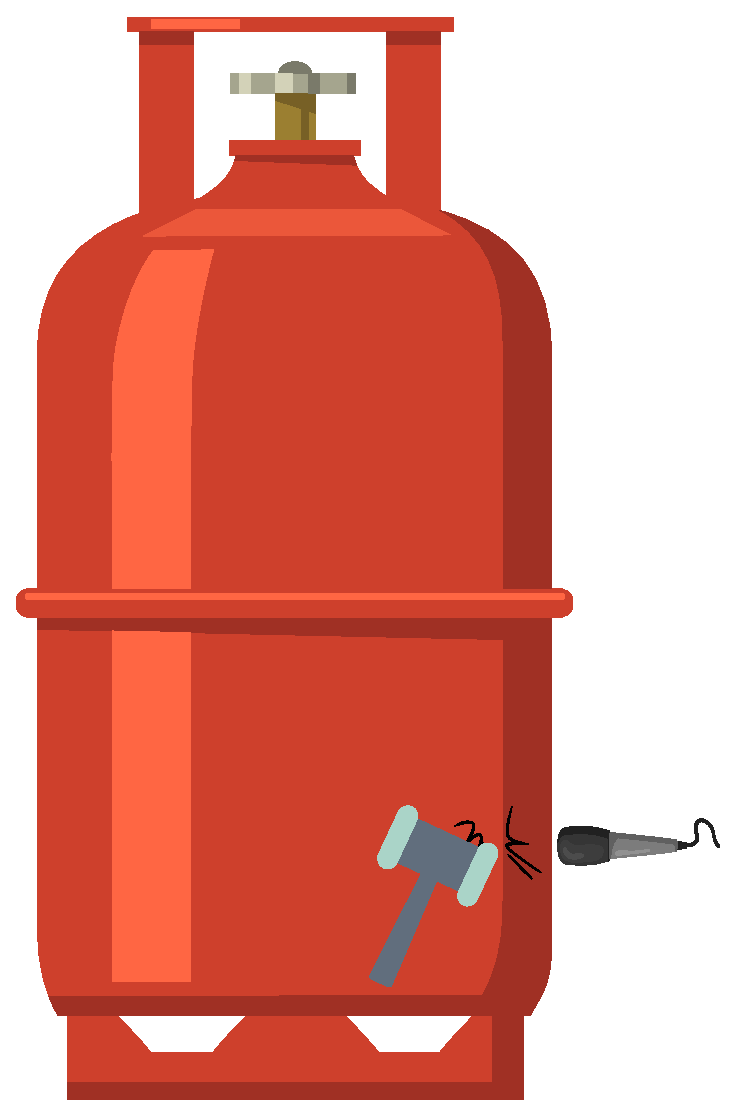
\includegraphics[width=0.3\textwidth]{Chapters/4CHP/Figures/micWimpactHamm.eps}
    \caption{Illustration of the accelerometer mount with a load strap}
    \label{fig:micmount}
\end{figure}
In the practical setup, since it uses the microphone from the phone, the side of the phone where the microphone is, should be faced to the \acrshort{lpg} bottle, usually the bottom part.
\subsection{Accelerometer}
When using an accelerometer for sensing vibration, there are different methods to mount it to the desired surface. In the industry, where accelerometers are used to measure vibrations of motors/machines, the accelerometer is mounted to the surface with a screw, allowing good contact with the surface. But in the application pretended is not possible to use that method, since that would imply the change in the structure of the tank and the accelerometer in use is not ready for a screw mount. Although the best results are obtained with a screw mount there are other methods to mount the accelerometer. 

One of the options is by using an adhesive, but in a practical mount the surface and the sensor would require different mounting bases, to avoid damaging the sensor and allow the sensor to be removed any time. Although this is practical to mount, it would also require that each tank already had the adhesive for the mount. The second option is a magnetic mount, offer a convenient mount if the structure of the tank is metallic. For this case it is advised that the magnet is in a separate piece, to avoid damaging the accelerometer. Magnets with a high pull strength are better in providing a good frequency response and a system with dual-magnet mount is good when the surface that the sensor is mounted on, is curve\cite{GuidelinesMountingTest}.

For the mount of the accelerometer in the \acrshort{lpg} bottle, will be used a magnet mount, is the most practical mount for a future application. Although in a laboratory environment and for test effects it will not be the only type of mount used. The first mount method will be with a load strap, this will hold firmly the sensor against the wall of the tank, as will be used for the first tests. In figure \ref{fig:mounLoadStrap} is an illustration of the sensor mount.

\begin{figure}[]
    \centering
    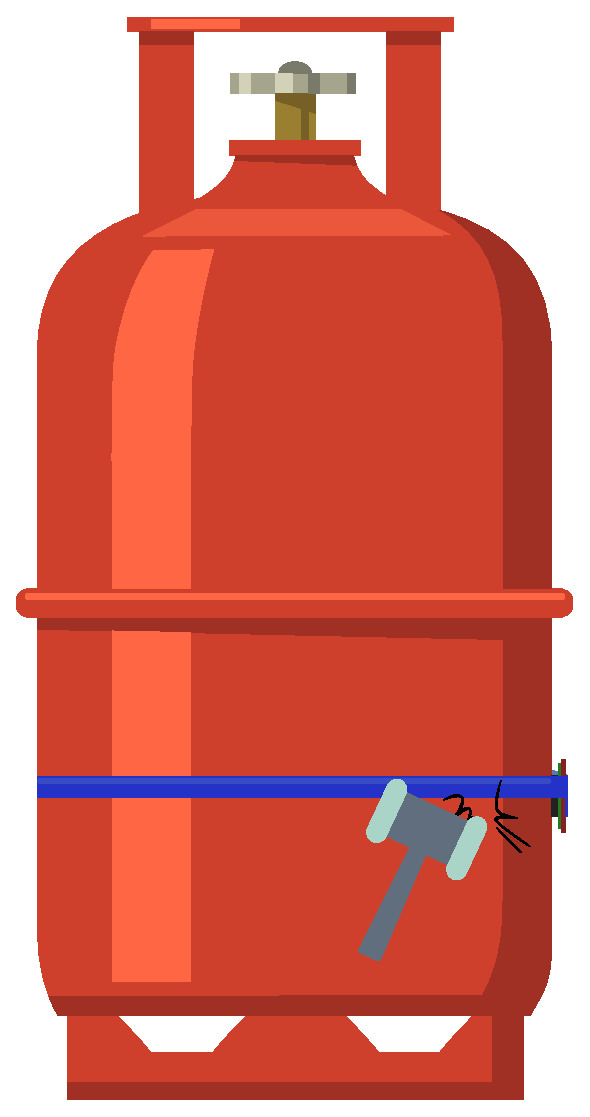
\includegraphics[width=0.3\textwidth]{Chapters/4CHP/Figures/AccLoadStrap.eps}
    \caption{Illustration of the accelerometer mount with a load strap}
    \label{fig:mounLoadStrap}
\end{figure}

For the magnet mount, there are actually two proposals, if by any reason one does not produce any results. In figure~\ref{subfig:mounMagnetDual} is the ideal option, since it is less invasive for the accelerometer, for the reason mentioned above. In this case, a piece is design to be able to mount with two neodymium magnets at the top and bottom of the piece, this will push the piece against the wall of the tank. Between the two magnets is the necessary space for held the accelerometer, a sponge will be glued to the piece on one side and the other will be glued to the accelerometer. This will be slightly thicker than the piece in that way when the magnets attached the piece against the tank wall, the sponge will be compressed and the surface of the accelerometer, is expected to be firmly held against the tank wall as well. In figure~\ref{subfig:mounMagnetsingle}, the mount is not ideal, since the neodymium magnet will be glued to the accelerometer surface for a god contact. This may result in better results when compared with the first option, but can damage the accelerometer, when attaching or removing the accelerometer from the tank wall.
\begin{figure}[]
    \centering
    \begin{subfigure}{0.3\textwidth}
        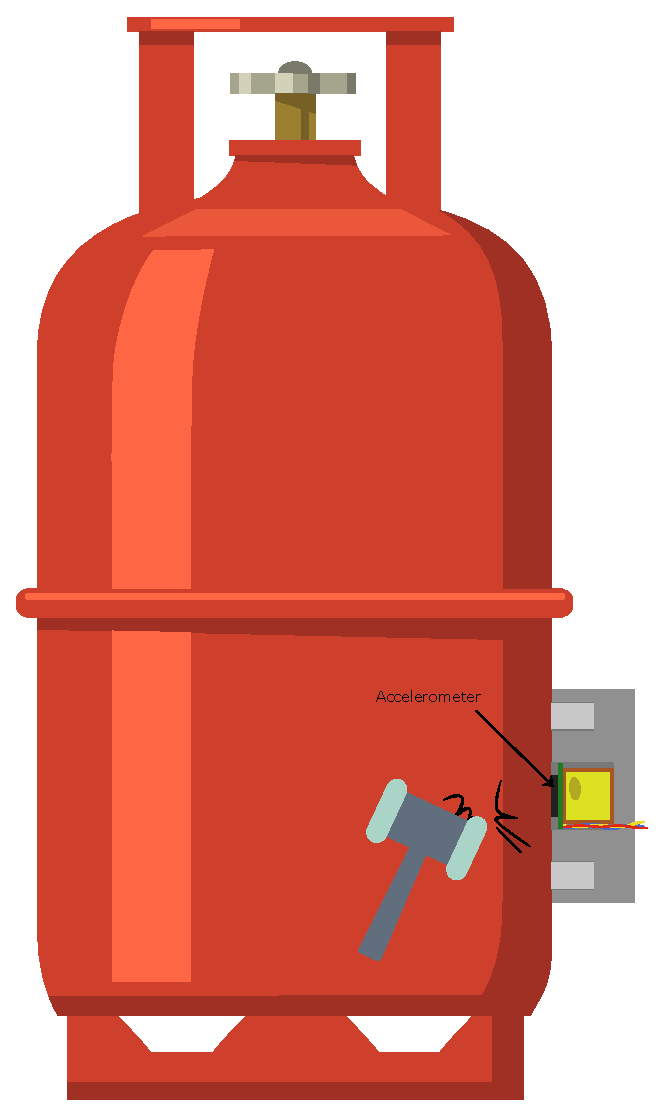
\includegraphics[width=\linewidth]{Chapters/4CHP/Figures/AccMagnets.eps}
        \caption{Illustration of dual-rail magnets mount}{}
        \label{subfig:mounMagnetDual}
    \end{subfigure}
    \begin{subfigure}{0.3\textwidth}
        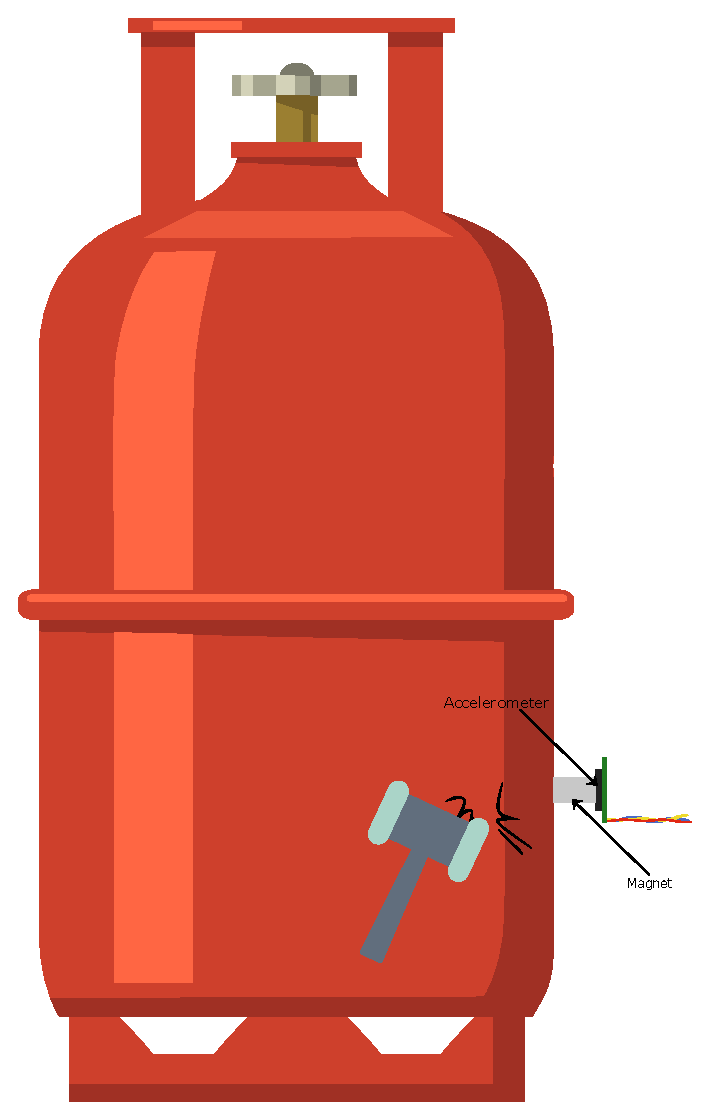
\includegraphics[width=\linewidth]{Chapters/4CHP/Figures/AccSMagnet.eps}
        \caption{Illustration of single magnet mount}{}
        \label{subfig:mounMagnetsingle}
    \end{subfigure}
    \caption{Illustration of the accelerometer mount with magnets}{}
    \label{fig:mounMagnet}
\end{figure}
%

\subsection{Piezoelectric}
\acrshort{ti} provides a document~\cite{minasiHowSelectMount2015}, with considerations for mounting a piezoelectric sensor to measure liquid level using ultrasonic waves. Although is a different approach, the key aspect for mounting this type of sensors can be used as well to define how to properly mount them. What needs to be taken into account, according to the document is, if the sensors is to be mounted inside or outside, at the top or at the bottom and for last the temperature range that the sensor can handles before starts to degrading the piezoelectric capability. It is quite clear the first aspect, since is suppose to be a non-invasive solution, which means that should be placed outside of the tank. The second aspect is not relevant since is being measured the vibration, not being used ultrasound to measure the liquid limit where the wave is reflected. The third aspect is also not that important since is expected to have the sensor at environment temperature unless, and this can be seen as an exception, when the gas from the tank has been release for a long period causing the outer wall of the bottle to freeze. Beside the first, which was already a requirement, none of the others will have a significant difference. For the purpose of measure through the walls of the tank is required to have a good contact between the transducer and the mounting surface. In their application the glue the transducer directly to the surface of the tank \cite{minasiHowSelectMount2015}.

Since the application is not ideal to have the transducer glued to the surface, the approach to have a good contact will be different, although the good results are not guaranteed. The figure \ref{fig:coupPiezo} is the illustration of two different mounting pieces for the transducer.
\begin{figure}[]
    \centering
    \begin{subfigure}{0.3\textwidth}
        \centering
        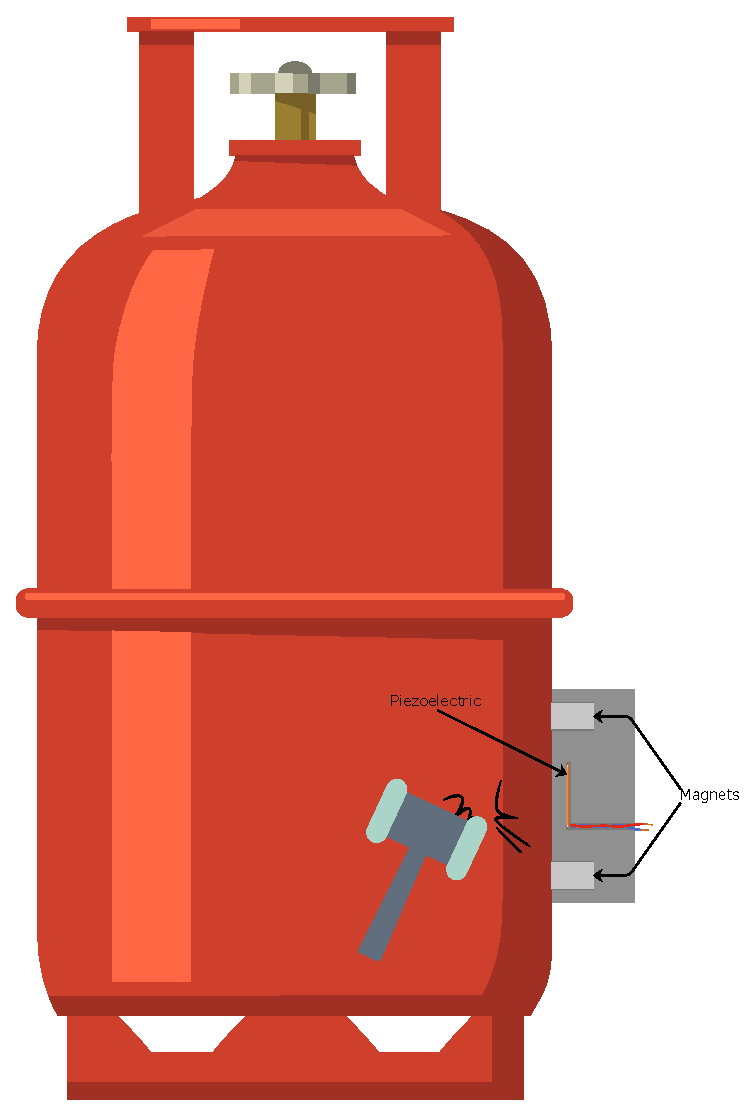
\includegraphics[width=\linewidth]{Chapters/4CHP/Figures/PiezoMagnetsSlot.eps}
        \caption{}{}
        \label{subfig:piezoslot}
    \end{subfigure}
    \begin{subfigure}{0.3\textwidth}
        \centering
        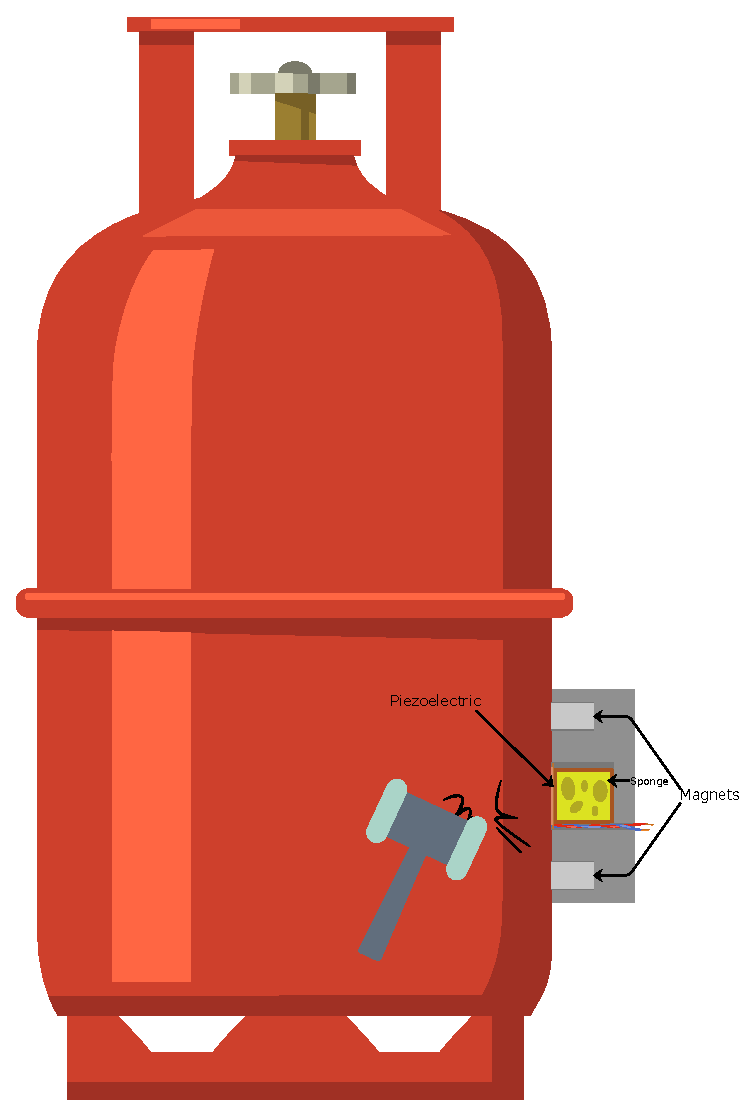
\includegraphics[width=\linewidth]{Chapters/4CHP/Figures/PiezoMagnets.eps}
        \caption{}{}
        \label{subfig:piezosponge}
    \end{subfigure}
    \caption{Illustration of the piezoelectric mount with magnets}{}
    \label{fig:coupPiezo}
\end{figure}

Both pieces will stay held to the tank with two magnets, one at the top of the piece and the other at the bottom. In figure \ref{fig:coupPiezo}~\subref{subfig:piezoslot}, the transducer is embedded in the piece, there is a slot in the middle, when the entire piece vibrates, the transducer vibrates with it. In the figure \ref{fig:coupPiezo}~\subref{subfig:piezosponge}, the coupling of the transducer is different when compared with the first one presented, the transducer is held glued to a sponge, and the sponge to the piece. The sponge is larger than the hole where the piece is glued in, so when the entire piece is attached to the walls of the tank, with the help of the magnets, it guarantees a good contact of the transducer with the wall. Since the sponge will press it against the wall and when there is vibration in the wall of the tank, it is expected to the transducer to capture the actual vibration. 

\section{Concluding remarks}
The current chapter presented the hardware parts and the physical components of the architecture presented to the system. The selection/design of the elements was based in already known concepts of electronics, properly justified, in most of the cases, with existing documentation about the topic.

The presented elements of hardware were either produced or prepared, to use in the step that follow this, i.e. the selected sensors were attached using the mentioned coupling methods, and the schematics presented were printed in a \acrshort{pcb}(\acrlong{pcb}), to use to drive required components of the system. These elements will later be part of the tests set, along with the software elements that will be explored in the next chapter.

\clearpage

%%%%%%%%%%%%%%%%%%%%%%%%%%%%%%%%%%%%%
% Developed Architecture
\cleardoublepage
\chapter{Software}
% To do: 
% Color Scheme
% Red - Not started
% Yellow - In progress
% Blue - Done, under approval
% Green - Done and approved
\todo[inline,color=red!40]{*Chapter Introduction}
\todo[inline,color=blue!40]{*1 - Microphone}
\todo[inline,color=yellow!40]{*2 - Microcontroller}
\todo[inline,color=blue!40]{ a) Peripherals}
\todo[inline,color=blue!40]{ b) FFT implementation}
\todo[inline,color=blue!40]{ c) Fixed-Point Square Root}
\todo[inline,color=red!40]{*3 - MatLab}
%%%%%%%%%%%%%%%%%%%%%%%%%%%%%%%%%% Writing %%%%%%%%%%%%%%%%%%%%%%%%%%%%%%%%%%%
%brief acknowledgment of what pieces are part of the developed software, add in the end a section how is intended to find the liquid level
\section{Microphone}
As the first measurements will be taken recurring to a microphone, it requires a different approach to the type of interaction when compared to the future application, were will be use a different sensor for the vibration. To obtain access and record the information from the microphone and for this case in specific, since is being used the microphone from a phone, will require different pieces of software to use in the phone side and the PC, to allow the access to the second to the microphone of the first. Also, on the PC side is necessary to record the information from the microphone and store it as desire.\\
The two components for this purpose will be the use of the WOMic software as the bridge between the phone and the computer, and MATLAB to record the information from the microphone. The second software can also be used to latter process the recorded data, helping the understand of the obtained information. 
\subsection*{WOMic}
The use of the application and the microphone of the phone is simple, although the installation and the configuration requires some time. For that, is required to install the software \textit{WOMic} in both devices, this allow to use the microphone of the phone in real-time. In the phone the software is available for Android and IOS and is responsible to transmit what is captured from the microphone, in the computer the client application and a virtual device must be installed to use the microphone in the PC to perform any type of tasks, this connection can be made over USB, Bluetooth, Wi-Fi and Wi-Fi Direct.\\ 
In order to save what is captured from the microphone, the software is split in three main block with different purposes, the \textit{WOMic App} runs in the phone, samples the input of the microphone and transmit it to the computer, the \textit{WOMic Client}, runs in the PC, connect to the app in the phone, and receive the data from the microphone, which is transmitted to the \textit{WOMic Virtual Device} on which a real microphone device is simulated and provides the audio to any application or program in the PC, as illustrated in figure \ref{fig:diagramWOMIC}.\\
\begin{figure}[!htb]
    \centering
    \includegraphics[width=0.65\textwidth]{Chapters/5CHP/Images/WOMICDiag.png}
    \caption{Flow of data in the components of the software}{\cite{WOMicFREE}}
    \label{fig:diagramWOMIC}
\end{figure}
In addition to this, is also necessary to install the drivers of the phone in use, if the connection is made over USB. To allow the access of the microphone in the PC, the transport mode must be selected on the phone application, USB in this case, in the app settings and after that start the application. In the PC the client software must be initialized and connected to the phone in the following order \textit{\>Connection\>Connect...} a new window will open, on which the USB must be selected as transport type and finalizing by pressing \textit{Connect}. With this, the microphone of the phone is available for use in the PC\cite{WOMicFREE}.
\section{Microcontroller}
%Introduction
%What is the purpose of each used element, Timer, UART, ADC, PINOUT for solenoid with timer
%What are the config of each
% Mainly from the ADC and how it works without having to use an additional timer
%
\subsection{Peripherals Configurations}
\subsubsection*{Timers}
In the configuration, two different timers were set, with the same configuration, one is used to measure the execution time of the algorithm and the other is used to set the amount of timer that the pin that triggers the solenoid is high. In this case were used Timer0\_A3 and Timer1\_A3, in both the counter mode of the timer is up, the division factor of the clock is 1 and they were set with a CCRx equal to 499, with this a interruption will occur at every 500$\mu$s.
\subsubsection*{ADC}
The LaunchPad in use offers ADC with a 10-bit, from the available pins, analog input 2 is selected. This input should be configured with the desire setting, to start is mandatory to disable the digital port of the pin to eliminate the flow of parasitic current flow, with the PySELx bits, by setting this bits HIGH it automatically enables the analog function of the port, although is still necessary to select the channel to conversion. The ADC will function in the sample and hold mode, using the timer from the ADC as the source of the sampling signal, the sample and hold period can be changed by software, to define the amount of clock cycles between each sample. 
\subsubsection*{eUSCI}
The eUSCI is used in UART mode to transfer data between the microcontroller and the PC, is used during the tests phase to perform two types of tests, one to test the algorithm and the other to receive data end send it to the PC. Both eUSCI\_A0 and eUSCI\_A1 support UART mode, unlike the eUSCI\_B0, the selected was the first, since works over the USB connection. In Transmission and Receiving, their were both set to work by polling with 115200bps of baud-rate, 8-bit, LSB first, no parity, no address and 1 stop bit.

\subsection{FFT implementation}
To process the signal captured from the ADC, is used a FFT algorithm. Two algorithms were considered to use in the microcontroller in use, a Fixed-Point and a Floating-Point versions, this algorithm was discovered by Cooley and Tukey in the beginning of the computer revolution and based on the complex DFT. The implementation used are based in FFT algorithm, and analysis the Fixed-Point and the Floating-Point side by side, they are quite similar, the main difference is in the data types used in each of the implementation, the fixed point can be adapted for the different types of signed integers, from 8-bits to 64-bits and uses a look-up table with the correspondent values of Sine and Cosine, used to calculate the real and imaginary in the frequency domain, this saves processing time, since isn't necessary to calculate these values while is the algorithm is running, on the other hand this limits the size of the vector to be processed, to be in maximum the size of the look-up table, unless the algorithm is adapted, this implementation is less time consuming for the microcontroller. The Floating-Point version calculates the values of the Sine and Cosine, and since it deals with values like float or double, which will require more memory and computational resources from the microcontroller if the same is used. Both implementation can be found on a repository in~\cite{262588213843476FixFft,Dannyf00FloatingPointFFTBenchmarka}, for a implementation from scratch there is also possible to find pseudo-code for that~\cite{smith1997scientist}.

The algorithms in use were adapted to fit in the purpose of the implementation for the microcontroller in use, as well as removed some option like the iFFT, which won't be necessary to use in this application.
\todo[inline,color=red!40]{Should I make a brief explanation of how the fft is implemented?}
After performing the FFT algorithm in the input data vector, is necessary to calculate the magnitude of the resulting data, since the algorithm returns complex values. To obtain the magnitude of the data in frequency is a simple mathematical operation and is described in~\ref{eq:magnitude}.
\begin{equation}\label{eq:magnitude}
    M = \sqrt{Re^2 + Im^2}
\end{equation}
\subsection{Fixed-Point Square Root}
For the application were the Fixed-Point is used is convenient to only deal with integers, after perform the FFT is necessary to calculate the magnitude of the signal, relative to the frequency, since the data returned from the algorithm is complex. For that as known, is necessary to use a the square root, several implementation of a Fixed-Point square root can be found, the implementation in use is an adaptation of the integer-to-integer version, from the repository~\cite{ChmikeFpsqrta}, in the used square root function, the input argument is a 32-bit value and the output a 16-bit value.

\section{MatLab}
This computational platform has various resources, with a lot appliances. For the purpose of the developed work only a few and simple function of this platform. In a initial stage, is going to be taken advantages of some of their function to generate random signals, in order to test the viability and precision of the FFT algorithm that will be used in a microcontroller environment, this requires the use of some basic mathematical functions and the serialport, the first is used to generate the random signal and the secondo to send the signal to to the microcontroller via UART, so it can be processed and the resulting data can be compared with the original. 

On other set of tests functions to record data from a certain audio input were used, to record the input of the microphone, each time that the LPG bottle is hit with the hammer. Beside this, the FFT function from the MATLAB is used to verify the response in frequency of the hit. 

Before the final application, is also need to verify the type of signals obtain in the sensors, after captured in the microcontroller the raw data is sent via UART to, once again, process them in the FFT function of MATLAB. 

\section{??}
% \begin{figure}[!htb]
%     \centering 
%         \begin{subfigure}[c]{\textwidth}
%             \centering
%             \input{Sections/3Transforms/Images/DFTSymmetry.tex}
%             \caption{}
%             \label{subfig:dft}
%         \end{subfigure}
%         \begin{subfigure}[c]{0.45\textwidth}
%             \centering
%             \input{Sections/3Transforms/Images/DCT1Symmetry.tex}
%             \caption{}
%             \label{subfig:dct1}
%         \end{subfigure}
%         \begin{subfigure}[c]{0.45\textwidth}
%             \centering
%             \input{Sections/3Transforms/Images/DCT2Symmetry.tex}
%             \caption{}
%             \label{subfig:dct2}
%         \end{subfigure}
%         \begin{subfigure}[c]{0.45\textwidth}
%             \centering
%             \input{Sections/3Transforms/Images/DCT3Symmetry.tex}
%             \caption{}
%             \label{subfig:dct3}
%         \end{subfigure}
%         \begin{subfigure}[c]{0.45\textwidth}
%             \centering
%             \input{Sections/3Transforms/Images/DCT4Symmetry.tex}
%             \caption{}
%             \label{subfig:dct4}
%         \end{subfigure}
%         \caption{Sequences generated in the first step of Table \ref{tab:DFTDCT}for the DFT and different DCTs. Filled dots correspond to the original sequence ((a) - \emph{DFT}; (b)) - \emph{DCT-I}; (c)) - \emph{DCT-II}; (d)) - \emph{DCT-III}; (e)) - \emph{DCT-IV}).}
%     \label{fig:2NSeq}
% \end{figure}
% \begin{lstlisting}
%     ./aomenc <INPUT-FILE> -h <HEIGHT> -w <WIDTH> -o <OUTPUT-FILE> --limit=10 -p 1 --cpu-used=8 --i420 --q-hist=64 --end-usage=q --cq-level=<CQ-LEVEL>
% \end{lstlisting}
%\addcontentsline{toc}{section}{References}

%%%%%%%%%%%%%%%%%%%%%%%%%%%%%%%%%%%%%
% Tests, Results and Analysis
\cleardoublepage
\chapter{Tests, Results and Analysis}\label{chap:Tests}
% To do: 
% Color Scheme
% Red - Not started
% Yellow - In progress
% Blue - Done, under approval
% Green - Done and approved
\todo[inline,color=red!40]{*Chapter Introduction}
\todo[inline,color=blue!40]{*1 - Algorithm Test}
\todo[inline,color=yellow!40]{*2 - Microphone Tests}
\todo[inline,color=red!40]{*3 - Accelerometer and PiezoElectric Tests}
%% Writing %%%%%%%%%%%%%%%%%%%%%%%%%%%%%%%%%%%%%%%%%%%%%%%%%%%%%%%%%%%%
\section{Algorithm Test}
The purpose of this, is to test the effectiveness of the algorithm implementation, mentioned in~\ref{subsec:fftImp}, one way to perform this test is recurring to random signals with known frequencies, this way is possible to compare the results from the implementation in a microcontroller environment with the absolute frequency determined when generation the random signal.

To try to perform the tests as close as possible to the type of signals that were expected to obtain, several aspects were taken into consideration, for that reason a small explanation of how the signals were generated will be given. 
%----------------Introduction above this line--------------------------
\subsection{Signal Generation}\label{subsec:sigGen}
To try to synthetize a wave form as similar as possible to the one resulting from the work of~\citeauthor{wuLiquidLevelDetector2014b} in figure~\ref{fig:realsignalWu}.
\begin{figure}[]
    \centering
    \begin{subfigure}{0.45\textwidth}
        \centering
        \includegraphics[width=\linewidth]{Chapters/6CHP/Figures/completesignalWu.pdf}
        \caption{Complete Signal}{}
        %\label{subfig:g1lines}
    \end{subfigure}
    \begin{subfigure}{0.45\textwidth}
        \centering
        \includegraphics[width=\linewidth]{Chapters/6CHP/Figures/fractionWu.pdf}
        \caption{Fraction of the signal}{}
        %\label{subfig:g2lines}
    \end{subfigure}
    \caption{Real signal}{~\cite{wuLiquidLevelDetector2014b}}
     \label{fig:realsignalWu}
 \end{figure}
First is randomly define a frequency to be the dominant and a regular wave was generated, to create the decay effect the resulting wave is multiplied by $\frac{1}{e^{x}}$ being $x=1$, creating the echo effect by adding the original wave multiplied by the same equation, increasing the value of $x$ and adding the wave to the original shifting N/16, with N being the original size of the wave. This procedure is repeated to generate more waves with different frequencies and smaller amplitudes, in the end random noise is added with random variance, being at maximum half of the signal generated without any noise. A example of the resulting waves can be observed in the figure~\ref{fig:synthetizedSignal}.
\begin{figure}[]
    \centering
    \begin{subfigure}{0.45\textwidth}
        \centering
        \includegraphics[width=\linewidth]{Chapters/6CHP/Figures/signal1.jpg}
        \caption{Noise variance of 0.05}{}
        %\label{subfig:g1lines}
    \end{subfigure}
    \begin{subfigure}{0.45\textwidth}
        \centering
        \includegraphics[width=\linewidth]{Chapters/6CHP/Figures/signal2.jpg}
        \caption{Noise variance of 0.01}{}
        %\label{subfig:g2lines}
    \end{subfigure}
    \begin{subfigure}{0.45\textwidth}
        \centering
        \includegraphics[width=\linewidth]{Chapters/6CHP/Figures/signal3.jpg}
        \caption{Noise variance of 0}{}
        %\label{subfig:g1lines}
    \end{subfigure}
    \begin{subfigure}{0.45\textwidth}
        \centering
        \includegraphics[width=\linewidth]{Chapters/6CHP/Figures/signal4.jpg}
        \caption{Noise variance of 0.5}{}
        %\label{subfig:g2lines}
    \end{subfigure}
    \caption{Example of signals synthetized with \acrshort{matlab} with different noise variances}{}
     \label{fig:synthetizedSignal}
 \end{figure}
\subsection{Tests}
To tests the effectiveness of the \acrshort{fft} algorithm in use, were perform in total 1000 tests to verify the obtained error of the implementation. The tests weren't only performed to the Fixed-Point algorithm in the microcontroller, the same code used in the microcontroller was also implemented in a \acrshort{pc} and the \acrshort{fft} function of \acrshort{matlab} was used as a control test, to verify that the signal wasn't to corrupted with noise that even \acrshort{matlab} wasn't able to determine the dominant frequency correctly.

In a \acrshort{pc} environment was implemented both \acrshort{fft}s, the Fixed-Point and the Floating-Point, in the microcontroller it was only possible to perform tests with the Fixed-Point since the other version exceeded the amount of memory needed to use the implementation. In each test a random signal was generated, as mentioned in~\ref{subsec:sigGen}, 512 samples of that signal were selected and converted to values between 0 and 1023, just like if it was converted by an \acrshort{adc}. After generating the signal, the dominant frequency is saved, to compare with the results, the samples are processed in \acrshort{matlab} and a dominant frequency is obtained and saved as well. The samples used in \acrshort{matlab} environment are saved, in order to be tested in both implementation in the \acrshort{pc} environment and the obtained results are saved. To finalize the samples are sent to the microcontroller and processed and the result is sent back to the \acrshort{pc} and saved. After all the tests, the results obtained are compared with the original value used in the frequency, allowing to verify how the algorithm performs. 
\begin{figure}[]
    \centering
    \includegraphics[width=1\textwidth]{Chapters/6CHP/Figures/ProcFlow.eps}
    \caption{Flow of signal processing in different environments}{}
    \label{fig:flowProc}
\end{figure}
Although the tests were perform in other environments, the test that is the most important is the one in the microcontroller. In the tests performed in the microcontroller not only the validity of the implementation, but is also necessary how long it takes to execute the algorithm in the microcontroller and what are the memory needs of the program. The program that executes the algorithm was built to start measuring the execution time of the \acrshort{fft} implementation right before it starts, and end it after calculated the magnitude of the resulting signal, to measure how long takes to perform these tasks it uses one of the timers that the microcontroller has. To better understand how all works, observe figure\ref{fig:dataProcuC}.
\begin{figure}[]
    \centering
    \includegraphics[width=1\textwidth]{Chapters/6CHP/Figures/uCDataProc.eps}
    \caption{Flow of processing in the microcontroller}{}
    \label{fig:dataProcuC}
\end{figure}
\subsection{Results}
The resulting data obtained is the dominant frequency of each implementation with the \acrshort{fft}, additionally in the microcontroller option was also measured the execution time of the algorithm. In the resulting dominant frequency from all cases was then compared with the absolute frequency, that was saved every time that a new signal was generated, the error obtained in each implementation can be observer in the table~\ref{tab:perfRes}.
\begin{table}
    \centering
    \includegraphics[width=1\textwidth]{Chapters/6CHP/Figures/performanceAlgorithm.pdf}
    \caption{Results of the execution of a synthetic signal in the different algorithms}
    \label{tab:perfRes}
\end{table}
Is evident that the results from \acrshort{matlab} are much better when compared with the rest and when comparing the Floating-Point with the Fixed-Point, in the \acrshort{pc} results, there is a slight difference between the two, but for the microcontroller in use wasn't possible to implement the Floating-Point, anyway the error obtained in the Fixed-Point doesn't increase significativily, with these results the use of the implementation is expected to be precise for the application. 

The results of the execution time of the algorithm can be observed in table~\ref{tab:excTimeuC}, the number of ticks is due the fact that to measure the execution time, a timer was configured to generate an interruption every 500$\mu$s, incrementing a variable each time that happen, as a result, by multiplying the number of ticks by the time each interruption is generated, gives the execution time of the algorithm. Taking into consideration that is microcontroller with a small processing power and the embedded Hardware Multiplier hasn't been used, around 3s to process 512 samples is acceptable, since isn't mandatory for the results to be returned in real-time.  
\begin{table}
    \centering
    \includegraphics[width=1\textwidth]{Chapters/6CHP/Figures/excTimeuC.pdf}
    \caption{Results of the execution of the Fixed-Point implementation in the microcontroller}
    \label{tab:excTimeuC}
\end{table}
%% Missing memory analysis, do that latter, se in code composer studio the indirect calls of the project
\section{Microphone Test}\label{sec:MicroTests}
\subsection{Signal Capturing and Tests}
%Topics to mention
% - The physical setup
% - How the data is captured with MatLab, also mentioned the sampling frequency
% - section mentioning the tests in different sports of the bottle, also mention the under case although wasn't tested
There are a few things that should be conclude from the tests with a microphone before starting the analysis with different sensors, they are in the first place the viability of the frequency analysis, for different liquid levels, if valid which is the frequency interval that should be taken into consideration and finally which are the more practical and were the best results are obtained, for latter help selecting the optimal point to place the sensor. 

Considering this, four points were considered to made some measurements, their identified in the illustration in figure~\ref{fig:measPointMic}, the points are all in the lateral surface of the \acrshort{lpg} bottle. The bottle in use is divided in two similar parts, by a welding joint in the middle, the lower and the top section, and the measuring points will be the bottom and the middle of each one of the sections, in other words, the points are right above the curvature and in the middle in the lower section and right above the welding joint and the middle of the top section. In some background studies made in chapter~\ref{chap:stArt}, another possibility was under the \acrshort{lpg} bottle but this option isn't practical, to place the microphone nor to hit the LPG bottle.
\begin{figure}[]
    \centering
    \includegraphics[width=0.35\textwidth]{Chapters/6CHP/Figures/measuringPointsMic.eps}
    \caption{Measuring points in the LPG bottle}{}
    \label{fig:measPointMic}
\end{figure}
In each of the points illustrated was recorded the sound produced when manual hitting the the lateral surface of the \acrshort{lpg} bottle, for the 3 bottles available. Each of the 3 bottles containing a different level of liquid, for safety reasons the liquid was water, and they were full, half-full and empty. 

To capture, record and save the sound, some of the \acrshort{matlab} capabilities were used to that purpose, the signal from the microphone was captured with a sampling frequency of 4k$Hz$, according to the table~\ref{tab:sampRat}, to ensure that there was enough time between setting the \acrshort{pc} to record and the manual hit, each saved sample is around 4 seconds, after it the signal can be processed and the resulting data analyzed.
%add here a flux gram
\subsection{Results}
%add images of the signals in the time domain
Several repetitions of the measurements were performed, to guarantee that the results obtained follow a determined pattern and won't vary much from one measurement to another. In the figure~\ref{fig:TimeRealDataMic} are presented the results from the different points of measurement in the different \acrshort{lpg} bottles and in figure~\ref{fig:ProcRealDataMic} the result from processing the same signals. Although is only presented one per point and bottle the remaining results were similar to the ones presented, the main difference for the remaining results can depend on how the hammer hits the surface of the LPG bottle and thus the signal can have smaller/bigger amplitude in the signals in the time domain, or peaks with higher/lower magnitude in the frequency domain.

%Time domain signals
\begin{figure}[]
    \centering
    \begin{subfigure}{0.45\textwidth}
        \centering
        \includegraphics[width=\linewidth]{Chapters/6CHP/Figures/TimeLowBottom.eps}
        \caption{Lower Section, Bottom Position}{}
        \label{subfig:timeLowBotMic}
    \end{subfigure}
    \begin{subfigure}{0.45\textwidth}
        \centering
        \includegraphics[width=\linewidth]{Chapters/6CHP/Figures/TimeLowCenter.eps}
        \caption{Lower Section, Center Position}{}
        \label{subfig:timeLowCenMic}
    \end{subfigure}
    \begin{subfigure}{0.45\textwidth}
        \centering
        \includegraphics[width=\linewidth]{Chapters/6CHP/Figures/TimeTopBottom.eps}
        \caption{Top Section, Bottom Position}{}
        \label{subfig:timeTopBotMic}
    \end{subfigure}
    \begin{subfigure}{0.45\textwidth}
        \centering
        \includegraphics[width=\linewidth]{Chapters/6CHP/Figures/TimeTopCenter.eps}
        \caption{Top Section, Center Position}{}
        \label{subfig:timeTopCenMic}
    \end{subfigure}
    \caption{Captured signals in different locations in the \acrshort{lpg} bottle}{}
     \label{fig:TimeRealDataMic}
\end{figure}

A example of how the hitting of the hammer affects the captured signal can be observed in the figure~\ref{subfig:timeLowCenMic}, where the signal from the empty bottle has a smaller amplitude when compared with the signals captured from the full/half bottle and in the figures~\ref{subfig:timeTopBotMic}\subref{subfig:timeTopCenMic} the same doesn't happen. For this reason, is also necessary to find alternatives to manual hitting in the \acrshort{lpg} bottle, first because the results won't be constant and second because in a final application is not practical to do it manually. But for know, the manual hitting was considered.

Even thought the time domain isn't considered to the detection of the liquid level, is interesting to observe the results obtained, beside the slight increase of the amplitude in the signal from the full bottle to the empty, the echo also increases in the same way as the amplitude, the the other difference is how long the echo/oscillation occurs, once again from the full bottle to the empty the interval of time that happens increases. 

%Latter correct the reference and sub reference above
%Frequency domain signals
\begin{figure}[]
    \centering
    \begin{subfigure}{0.45\textwidth}
        \centering
        \includegraphics[width=\linewidth]{Chapters/6CHP/Figures/LowBot.eps}
        \caption{Lower Section, Bottom Position}{}
        \label{subfig:LowBotMic}
    \end{subfigure}
    \begin{subfigure}{0.45\textwidth}
        \centering
        \includegraphics[width=\linewidth]{Chapters/6CHP/Figures/LowCenter.eps}
        \caption{Lower Section, Center Position}{}
        \label{subfig:LowCenMic}
    \end{subfigure}
    \begin{subfigure}{0.45\textwidth}
        \centering
        \includegraphics[width=\linewidth]{Chapters/6CHP/Figures/TopBot.eps}
        \caption{Top Section, Bottom Position}{}
        \label{subfig:TopBotMic}
    \end{subfigure}
    \begin{subfigure}{0.45\textwidth}
        \centering
        \includegraphics[width=\linewidth]{Chapters/6CHP/Figures/TopCenter.eps}
        \caption{Top Section, Center Position}{}
        \label{subfig:TopCenMic}
    \end{subfigure}
    \caption{Processed Signals in different locations in the \acrshort{lpg} bottle}{}
     \label{fig:ProcRealDataMic}
\end{figure}

After processing the data from the results obtained, observed in the figure~\ref{fig:ProcRealDataMic}, one obvious conclusion is that the signal measured ate the lower section in the bottom, in figures\ref{subfig:timeLowBotMic} and~\ref{subfig:LowBotMic} doesn't result in a signal with the same amplitude in the time domain nor the same magnitude in the frequency domain, for analysis of the results this point was discarded. From the remaining points they both show some similarities, with the best results obtained in the top section in the center\ref{subfig:TopCenMic}. Comparing the lower section in the center and the top section in the bottom, the results are slightly better in the second point mentioned, although for future measurements, the point considered will depend in the results obtained when changing the sensor in use.

To reduce the amount of time used in the identification of the liquid level, is interesting to be able to determine a frequency interval to search, the limits of the interval should be determine by the response in frequency of a full and a empty \acrshort{lpg} bottle. The results obtained from the points considered show that, isn't identify for the full bottle any frequency in the systems response bellow the $+/-700Hz$, for the other two bottles this value increases, for the bottle half filled the value shifts to $+/-800Hz$ and for the empty bottle to $+/-900Hz$, with this in mind the lower limit for the searching interval can be set around $+/-650Hz$, to have a margin. This shift in frequency from one bottle to another can considered as a identification method, since the first peak occurs, according to the obtained results, between the $700Hz$ to $900Hz$. 

From the first peak observed in the system response, is visible the increase in magnitude of the following peaks, until reaches a certain value were starts to decreases again, where starts to increase once again. Where the pattern starts to repeat, can be defined as the limit of searching. If observed, starts to repeat around $400Hz$ after the first peak is identified, this can be used in combination to the identification of the first peak to check if after $+/-400Hz$, the identified peak has a higher magnitude than the previous, meaning that the pattern is repeating once again. 

Another thing that is characteristic in the response to a stimulation of each bottle, is observed that the peak with the highest magnitude also shifts in frequency, in the interval of $+/-400Hz$ this value is approximately in the middle of this interval. For instance, for the full bottle the highest peak is around $800Hz$ and for the empty bottle is around $1100Hz$. Note that this results apply only for the results obtained at the top section and this identification method is the most inconstant, probably due the fact that the hitting is manual. Although this is not as certain as the mentioned before, this peaks also shift in frequency, which means that the searching for a peak in this interval is also valid for the liquid level identification, if combined with the the other characteristics identified.

Another characteristic that must be taken in consideration, not specific to the identification, is the smaller peaks that may appear close to the ones registered, with smaller magnitude, but if what is near each one of the peaks as a sum of the surrounding, may help in the identification, this isn't mandatory to use in the identification but must be considered when developing the method to identify the liquid level.
%% Is really necessary?
To sum-up, in the development of a method to identify the liquid level should be considered the following three characteristics:
\begin{itemize}
    \item The interval on which the first peak will appear, between $650Hz$ and $950Hz$ approximately;
    \item The frequency were starts the repetition pattern, around $400Hz$ after appearing the first peak;
    \item The interval on which the peaks with the highest magnitude appears, between $800Hz$ and $1100Hz$ approximately. 
\end{itemize}

\section{Accelerometer and PiezoElectric Tests}

In chapter ~\ref{chap:hardware}, section ~\ref{sec:CaptureCoupling} is presented several methods to mount the sensors were presented. From those, it was selected 3 different methods to mount the accelerometer in the \acrshort{lpg} and 2 for the piezoelectric. The purpose of this is to test the sensors and find the most reliable mount method, to measure the liquid level.

Beside the mounting method is important to verify how the stimulation of the bottle affects the response of the system and thus the obtained results from the sensors in use. Considering this, in the performed measurements, the stimulation was always in two different ways, manually with a hammer hitting the surface of the \acrshort{lpg}, and automatically with a impulse created with a solenoid.

The setups in the measurements, for the different stimulation methods, will be explained and the results obtained for each one of them will be analyzed in the continuation of this section.
\subsection{Stimulation and Vibration Measuring}
%Explain why only 2 stops for measurements were considered
Even though that in section ~\ref{sec:MicroTests} of this chapter, was considered four different points to perform measurements, in this case it was considered only two of those four point, mainly due the fact that for the dual magnet mount it wasn't practical to place the printed piece in the bottle. From the measuring points presented in figure ~\ref{fig:measPointMic}, was only considered the center points in both lower and top sections of the bottle.

%In both cases, manual or automatic, the software used is the same in both sensors used. 
The configurations used to sampling the signal for the different sensors were similar, since both amplifier circuit have their output centered in half of the supply voltage. So, in each one of the sampling manners used to sampling the signals, refer to the both cases. 
% Explain how the signal is capture when Manual
%\subsubsection*{Manual Stimulation}

% Explain how the signal is capture when automatic
%\subsubsection*{Automatic Stimulation}
 
\begin{description}
    \item[Manual Stimulation]{- After configuring all the peripherals necessary, a externa interruption is set to be trigger with a push-button, when pressed it enables the timer to control the sampling frequency, and starts to read the value from the analog input. The read values aren't stored right away, waits until a certain input value is reached, it is set to be under/above 128 from the mid value, this value is only passed if we knock on the bottle. From this point 1024 samples are stored and then sent via \acrshort{uart} to the computer.}
      
    \item[Automatic Stimulation]{- Similar to the manual stimulation read, the peripherals are configured and the same external interruption is set. When pushed, the interruption will activate a timer that actuates in the solenoid, simulating the impulse desire to stimulate the system. Right after stimulation the system, the timer responsible for the sampling, is activated and the conversion starts, storing 1024 samples, which are send via \acrshort{uart} to the computer.} 

\end{description}
On the computer side, the data is received from \acrshort{uart} and stored with the use of \acrshort{matlab}. In order to analyze the data acquired with the sensors, first is used \acrshort{matlab}, that allows for a faster method to process the data and plot the results for the analysis. Before process the data in the \acrshort{fft} algorithm implemented in the microcontroller, a visual analysis must be performed to verify what are the the characteristics of the processed signals, in each configuration, to later identify what is the proper method to identify the liquid level.  
%Draw fluxograms
%Explain how the data will be analyzed in the matlab
\subsection{Results}
From the Sensors used several measurements where performed, in the different locations, configurations and stimulations. The considered aspects for the measurements, although already mentioned previously, where done as follows:
\begin{enumerate}
    \item The measuring Point
    \begin{enumerate}
        \item Center, Lower Section;
        \item Center, Upper Section;
    \end{enumerate}
    \item The Stimulation Method
    \begin{enumerate}
        \item Manual, with a hammer;
        \item Automatic, with a solenoid;
    \end{enumerate}
    \item The Sensors
    \begin{enumerate}
        \item Small PiezoElectric with the sponge;
        \item PiezoElectric in a slot inside the piece;
        \item Accelerometer with the sponge;
        \item Accelerometer attached to the bottle with a magnet;
        \item Accelerometer attached to the bottle with a load strap; 
    \end{enumerate}
\end{enumerate}
From the combination of all this aspects, the results obtained are the following:
%plot the results One sensor at a time with automatic and manual side by side, the first 2 the lower section, the second 2 the top section
% LOW Manual || LOW Automatic
% UP Manual  || UP Automatic
%Accelerometer load strap
\begin{figure}[]
    \centering
    %Low
    \begin{subfigure}{0.45\textwidth}
        \centering
        \includegraphics[width=\linewidth]{Chapters/6CHP/Figures/ResultsSensors/AcCiMaBot.pdf}
        \caption{Manual Stimulation at the center of the lower section}{}
        \label{subfig:ResAcCiMaBot}
    \end{subfigure}
    \begin{subfigure}{0.45\textwidth}
        \centering
        \includegraphics[width=\linewidth]{Chapters/6CHP/Figures/ResultsSensors/AcCiAuBot.pdf}
        \caption{Automatic Stimulation at the center of the lower section}{}
        \label{subfig:ResAcCiAuBot}
    \end{subfigure}
    %Up
    \begin{subfigure}{0.45\textwidth}
        \centering
        \includegraphics[width=\linewidth]{Chapters/6CHP/Figures/ResultsSensors/AcCiMaTop.pdf}
        \caption{Manual Stimulation at the center of the upper section}{}
        \label{subfig:ResAcCiMaTop}
    \end{subfigure}
    \begin{subfigure}{0.45\textwidth}
        \centering
        \includegraphics[width=\linewidth]{Chapters/6CHP/Figures/ResultsSensors/AcCiAuTop.pdf}
        \caption{Automatic Stimulation at the center of the upper section}{}
        \label{subfig:ResAcCiMaTop}
    \end{subfigure}
    \caption{Accelerometer attached to the bottle with a load strap}{}
    \label{fig:AccLoadStrap}
\end{figure}
%Accelerometer magnet
\begin{figure}[]
    \centering
    %Low
    \begin{subfigure}{0.45\textwidth}
        \centering
        \includegraphics[width=\linewidth]{Chapters/6CHP/Figures/ResultsSensors/AcImMaBot.pdf}
        \caption{Manual Stimulation at the center of the lower section}{}
        \label{subfig:ResAcImMaBot}
    \end{subfigure}
    \begin{subfigure}{0.45\textwidth}
        \centering
        \includegraphics[width=\linewidth]{Chapters/6CHP/Figures/ResultsSensors/AcImAuBot.pdf}
        \caption{Automatic Stimulation at the center of the lower section}{}
        \label{subfig:ResAcImAuBot}
    \end{subfigure}
    %Up
    \begin{subfigure}{0.45\textwidth}
        \centering
        \includegraphics[width=\linewidth]{Chapters/6CHP/Figures/ResultsSensors/AcImMaTop.pdf}
        \caption{Manual Stimulation at the center of the upper section}{}
        \label{subfig:ResAcImMaTop}
    \end{subfigure}
    \begin{subfigure}{0.45\textwidth}
        \centering
        \includegraphics[width=\linewidth]{Chapters/6CHP/Figures/ResultsSensors/AcImAuTop.pdf}
        \caption{Automatic Stimulation at the center of the upper section}{}
        \label{subfig:ResAcImAuTop}
    \end{subfigure}
    \caption{Accelerometer attached to the bottle with a magnet}{}
    \label{fig:AccMagnet}
\end{figure}
%Accelerometer sponge
\begin{figure}[]
    \centering
    %Low
    \begin{subfigure}{0.45\textwidth}
        \centering
        \includegraphics[width=\linewidth]{Chapters/6CHP/Figures/ResultsSensors/AcEsMaBot.pdf}
        \caption{Manual Stimulation at the center of the lower section}{}
        \label{subfig:ResAcEsMaBot}
    \end{subfigure}
    \begin{subfigure}{0.45\textwidth}
        \centering
        \includegraphics[width=\linewidth]{Chapters/6CHP/Figures/ResultsSensors/AcEsAuBot.pdf}
        \caption{Automatic Stimulation at the center of the lower section}{}
        \label{subfig:ResAcEsAuBot}
    \end{subfigure}
    %Up
    \begin{subfigure}{0.45\textwidth}
        \centering
        \includegraphics[width=\linewidth]{Chapters/6CHP/Figures/ResultsSensors/AcEsMaTop.pdf}
        \caption{Manual Stimulation at the center of the upper section}{}
        \label{subfig:ResAcEsMaTop}
    \end{subfigure}
    \begin{subfigure}{0.45\textwidth}
        \centering
        \includegraphics[width=\linewidth]{Chapters/6CHP/Figures/ResultsSensors/AcEsAuTop.pdf}
        \caption{Accelerometer attached to the bottle with a load strap}{}
        \label{subfig:ResAcEsAuTop}
    \end{subfigure}
    \caption{Accelerometer attached to the bottle with a dual mount magnet and a sponge}{}
    \label{fig:AccSponge}
\end{figure}
%Piezo Big
\begin{figure}[]
    \centering
    %Low
    \begin{subfigure}{0.45\textwidth}
        \centering
        \includegraphics[width=\linewidth]{Chapters/6CHP/Figures/ResultsSensors/PiezBMaBot.pdf}
        \caption{Manual Stimulation at the center of the lower section}{}
        \label{subfig:ResPiezBMaBot}
    \end{subfigure}
    \begin{subfigure}{0.45\textwidth}
        \centering
        \includegraphics[width=\linewidth]{Chapters/6CHP/Figures/ResultsSensors/PiezBAuBot.pdf}
        \caption{Automatic Stimulation at the center of the lower section}{}
        \label{subfig:ResPiezBAuBot}
    \end{subfigure}
    %Up
    \begin{subfigure}{0.45\textwidth}
        \centering
        \includegraphics[width=\linewidth]{Chapters/6CHP/Figures/ResultsSensors/PiezBMaTop.pdf}
        \caption{Manual Stimulation at the center of the upper section}{}
        \label{subfig:ResPiezBMaTop}
    \end{subfigure}
    \begin{subfigure}{0.45\textwidth}
        \centering
        \includegraphics[width=\linewidth]{Chapters/6CHP/Figures/ResultsSensors/PiezBAuTop.pdf}
        \caption{Accelerometer attached to the bottle with a load strap}{}
        \label{subfig:ResPiezBAuTop}
    \end{subfigure}
    \caption{Big PiezoElectric inserted in a slot of a dual mount magnet piece}{}
    \label{fig:PiezB}
\end{figure}
%piezo small
\begin{figure}[]
    \centering
    %Low
    \begin{subfigure}{0.45\textwidth}
        \centering
        \includegraphics[width=\linewidth]{Chapters/6CHP/Figures/ResultsSensors/PiezzMaBot.pdf}
        \caption{Manual Stimulation at the center of the lower section}{}
        \label{subfig:ResPiezzMaBot}
    \end{subfigure}
    \begin{subfigure}{0.45\textwidth}
        \centering
        \includegraphics[width=\linewidth]{Chapters/6CHP/Figures/ResultsSensors/PiezzAuBot.pdf}
        \caption{Automatic Stimulation at the center of the lower section}{}
        \label{subfig:ResPiezzAuBot}
    \end{subfigure}
    % Up
    \begin{subfigure}{0.45\textwidth}
        \centering
        \includegraphics[width=\linewidth]{Chapters/6CHP/Figures/ResultsSensors/PiezzMaTop.pdf}
        \caption{Manual Stimulation at the center of the upper section}{}
        \label{subfig:ResPiezzMaTop}
    \end{subfigure}
    \begin{subfigure}{0.45\textwidth}
        \centering
        \includegraphics[width=\linewidth]{Chapters/6CHP/Figures/ResultsSensors/PiezzAuTop.pdf}
        \caption{Accelerometer attached to the bottle with a load strap}{}
        \label{subfig:ResPiezzAuTop}
    \end{subfigure}
    \caption{Small PiezoElectric attached with a dual magnet mount and a sponge}{}
    \label{fig:Piezz}
\end{figure}
% analyze the results
\todo[inline,color=red!40]{*Add link to the remaining results if necessary and addapt the first paragraph that follows to lead to the results latter!}
Note that the presented results in the images above, are only referring to one sample of each bottle in each setup. In overall were performed at least 10 measurements in each point and setups, most of the measurements repeated more than once with small adjustments, at the hardware or software. The presented ones refer to the last series of measurements. %Add reference to the folder were are the remaining results??

From all the results presented for the different setups, one thing is clear, the use of the solenoid for the automatic stimulation was a complete failure, none of the presented graphics on that setup provided relevant information about the liquid level, this lead to the conclusion that the stimulation with the solenoid isn't enough to the accelerometer or the piezoelectric sensor determine the variation in vibration for the different bottles, as is going to be proved when analyzing the manual stimulation. 

This may be due the fact that the impact caused with the solenoid isn't enough to produce a visible vibration of the systems that surpasses the natural oscillation of the output of the sensors, that after being amplified results in noise. Although a the noise is a problem, this could be bypassed by averaging, different spectrums of different measurements in the same conditions, this results in a decrease of the noise but without the expected results, the spectrum obtain still returned random values, without clear information.

From the results obtained with the manual stimulation, the conclusions are the same as above, with two exceptions. Those were by using the accelerometer attached with a load strap and one magnet. From these two, the most clear results are in the accelerometer attached with a load strap, but is also visible a pattern between the three bottles, with the first highest peaks occurring between $+/- 700Hz$ to the $+/-900Hz$, from the full to the empty bottle. The same results are also visible with the magnet, but with the introduction of more peaks in between with smaller amplitudes, this is reduced when averaging the spectrum.

Another thing that is important to mentioned is that even though several measurements with the piezoelectric were performed, none of them presented relevant information, not even when averaging the spectrum. In the different tests was never clear what was the reason why the piezoelectric haven't any valid results. 
%conclusions
Considering the presented setups, is only going to be used in future analysis the two setups that have show some results, that are the accelerometer with one magnet and the load strap. One final conclusion to take from all performed measurements, is how much the impact affects the response of the system and thus the acquired signal with the sensor, as well as the mounting of the sensor plays an important role in the captured vibration.
\section{Identification algorithm Tests}
% what signals where considered
At this stage is important to move from the tests and analysis with \acrshort{matlab} and verify if the algorithm implemented in the microcontroller returns similar results, for this were considered the signals obtained with the microphone, the accelerometer with the load strap and the accelerometer with the magnet. The signals captures with the microphone were used because their spectrum was less noisy than the spectrum from the other sensors, if the identification didn't work with these signals, it wouldn't for sure to work with the remaining. Also, they were used as a way to define the limits of search in the identification algorithm, i.e. to define the interval in frequency to the identification of the liquid level.  
% How the tests were performed
\subsection{Identification Steps??}
The first step was to obtain the spectrum of signals from the three different bottles, to define the interval in frequency in order to reduce the amount of time in the search having more accuracy. In this case, the original signal was cropped and send to the microcontroller for processing, returning then to the computer for analysis.
After this, a interval was determined and the identification algorithm was developed to find the liquid level. What it does is, a threshold value is determined between a relation of the average amplitude of the spectrum and the highest peak, this allow for the threshold value to vary according to the amplitude of the signal. This threshold value is what determines if is a important peak, or is just noise related. 

Considering this threshold value and the limits defined, three main functions were created. The first one identifies the first peak, starts to look in the lower limit and goes until a upper limit, when find the first value above the threshold value, the function stops and returns the value.
The second function considers a different limit, the lower is the same as in the first situation, the upper is set according to the cutoff frequency of the accelerometer, when testing with their values, otherwise is set until half of the sampling frequency. This function finds the highest peak in the spectrum, search for the intire spectrum considered and when ends returns the value of the highest one.
The third function was developed, to try bypass one thing that was noticed in the second, most of the times the highest peaks matches with the first peak, which is due the inconsisty of the knock. When this occurs, near the frequency were it usually occurs, the spectrum has smaller peaks around it instead of a highest one, this was the way to try to find the consisty, by averaging around each peak and determine which one of them has the highest energy. The purpose of this third function is exactly this and return the value of were this happens.

Considering the functions for the identification of the liquid level, the signals obtained with the microphone, and the two configurations with the accelerometer, were sent to the microcontroller for identification and processing and the results of the identification return to the computer. On the computer side is the results were plotted in order to find how well the identification functions worked. 

One thing important to mentioned is, the only reason that the definition of the threshold value is this way is, since the manual hitting produces different responses, the algorithm needs to adapt to that variation, if the process was automatic this probably wouldn't be necessary, was expected to have consistence between all the signal captured to the same point.  
\subsection{Results}
% Add a graphics with the spectrum of the signals from the microphone obtained in the microcontroller  
%% add the rest tomorrow


\clearpage
%\printbibliography[heading=subbibliography]
%\addcontentsline{toc}{section}{References}


%%%%%%%%%%%%%%%%%%%%%%%%%%%%%%%%%%%%%
% Developed Architecture
%\cleardoublepage
\renewcommand{\thesection}{\Alph{section}}
\begin{appendices}

%%\section{\emph{aomenc} Configuration Options} \label{app:libaom}
%%\begin{lstlisting}
%%\end{lstlisting}

%%%%%%%%%%%%%%%%%%%%%%%%%%%%%%%%%%%%%%%%%%%%%%%%%%%%%%%%%%%%%%%%%%%%%%%%%%%
%%\section{DCT8\_1 VHDL Description} \label{app:dct81}
%%\begin{lstlisting}[style=vhdl]
%%\end{lstlisting}

%%%%%%%%%%%%%%%%%%%%%%%%%%%%%%%%%%%%%%%%%%%%%%%%%%%%%%%%%%%%%%%%%%%%%%%%%%%
%%\section{DCT8\_2 VHDL Description} \label{app:dct82}
%%\begin{lstlisting}[style=vhdl]
%% \end{lstlisting}
\end{appendices}


%%%%%%%%%%%%%%%%%%%%%%%%%%%%%%%%%%%%%
% Bibliography
%\cleardoublepage
%  \nocite{*}
%  \printbibliography
%\cleardoublepage

\end{document}
